\documentclass[10pt,journal,compsoc]{IEEEtran}
\usepackage{alltt}
\usepackage{multirow}
\usepackage{graphicx}
\usepackage{color}
\usepackage[labelfont=bf,textfont={bf}]{caption}
\usepackage{subcaption}
\usepackage{pifont}% http://ctan.org/pkg/pifont
\usepackage{boxedminipage}
\usepackage{notoccite}
\usepackage{array}
\newcolumntype{C}[1]{>{\centering\let\newline\\\arraybackslash\hspace{0pt}}m{#1}}
\usepackage{enumerate}
\usepackage{booktabs}
\usepackage{minted}
\usepackage[framemethod=tikz]{mdframed}
\usepackage{lipsum}
\usetikzlibrary{shadows}
\usepackage{mathtools}
 \usepackage{paralist}
 \definecolor{light-gray}{gray}{0.80}
\usepackage{graphics}
\usepackage[shortlabels]{enumitem}
%\usepackage{balance}
\usepackage{dblfloatfix}

%\usepackage{hyperref}
%\usepackage{cleveref}
\usepackage{colortbl}
\newmdenv[
  tikzsetting= {fill=light-gray},
  linewidth=1pt,
  roundcorner=0pt, 
  shadow=false
]{myshadowbox}
\usepackage{colortbl} 
\usepackage{subcaption}
\usepackage{blindtext, graphicx}
\usepackage{textcomp}
\usepackage{mathtools}
\usepackage[hidelinks]{hyperref}
\usepackage{amsmath}
\usepackage{amsfonts}
\usepackage{caption}
\usepackage{color}
\usepackage[final]{listings}
\usepackage{graphicx} 
\usepackage{multirow}
\usepackage{balance}
\usepackage{picture}
\usepackage{relsize}
\usepackage{multicol}
\usepackage{soul}
\usepackage{enumitem}
\setitemize{noitemsep,topsep=0pt,parsep=0pt,partopsep=0pt,leftmargin=*}
\setenumerate{noitemsep,topsep=0pt,parsep=0pt,partopsep=0pt,leftmargin=*}
\DeclarePairedDelimiter\abs{\lvert}{\rvert}%
\usepackage{array}
\usepackage{makecell}
\usepackage{bigstrut}
\newcommand{\tion}[1]{\S\ref{sect:#1}}
\newcommand{\fig}[1]{Figure~\ref{fig:#1}}
\newcommand{\tab}[1]{Table~\ref{tab:#1}}
\definecolor{comment_color}{rgb}{0.5, 0, 1}
\definecolor{steel}{rgb}{0.1, 0.3, 0.5} 
\newcommand{\cmark}{\ding{51}}%
\newcommand{\xmark}{\ding{55}}%
\newcommand{\todoc}[2]{{\textcolor{#1}{\textbf{[[#2]]}}}}
\newcommand{\todobrown}[1]{\todoc{green}{\textbf{[[#1]]}}}
\newcommand{\todoblue}[1]{\todoc{blue}{\textbf{[[#1]]}}}
\newcommand{\todoorange}[1]{\todoc{cyan}{\textbf{[[#1]]}}}
\newcommand{\todored}[1]{\todoc{red}{\textbf{[[#1]]}}}
\newcommand{\rahul}[1]{{\textcolor{steel}{#1}}}
\newcommand{\bi}{\begin{itemize}}
\newcommand{\ei}{\end{itemize}}
\usepackage[
 pass,% keep layout unchanged
 % showframe,% show the layout
]{geometry}
\usepackage[skins]{tcolorbox}
\usepackage{verbatim}
\usepackage{algorithm}
\usepackage{algorithmicx}
\usepackage{algpseudocode}
\usepackage[export]{adjustbox}
\usepackage{mathtools}
\setlength{\belowcaptionskip}{-10pt}
\renewcommand{\footnotesize}{\scriptsize}
\renewcommand{\algorithmicrequire}{\textbf{Input:}}
\renewcommand{\algorithmicensure}{\textbf{Output:}}
\definecolor{lightgray}{gray}{0.8}
\definecolor{LightCyan}{rgb}{0.88,1,1}
\definecolor{darkgray}{gray}{0.6}
\definecolor{Gray}{rgb}{0.88,1,1}
\definecolor{Gray}{gray}{0.85}
\definecolor{Blue}{RGB}{0,29,193}
\definecolor{MyDarkBlue}{rgb}{0,0.08,0.45} 
\definecolor{pink}{RGB}{231,95,110}
\definecolor{lightergray}{rgb}{0.85, 0.85, 0.85}
\definecolor{lightestgray}{rgb}{0.95, 0.95, 0.95}
\definecolor{ao(english)}{rgb}{0.0, 0.5, 0.0}
% \frenchspacing
\lstset{
  language=Python,
  basicstyle=\sffamily\fontsize{2.5mm}{0.8em}\selectfont,
  breaklines=true,
  prebreak=\raisebox{0ex}[0ex][0ex]{\ensuremath{\hookleftarrow}},
  frame=l,
  showtabs=true,
  columns=fullflexible,
  showspaces=false,
  showstringspaces=false,
  keywordstyle=\color{pink}\bfseries\sffamily\fontsize{2.8mm}{0.6em},
  emph={train, predict, add_samples, FindBellwether, BEETLE, get_cost, sample, get_perf, remove_non_bellwethers, LinearTransform, GPTransform}, 
  emphstyle=\bfseries\color{black!80} ,
  stringstyle=\itshape\color{black!50},
  commentstyle=\color{red!50!black}\it,
  numbers=left,
  captionpos=t,
  escapeinside={\%*}{*)}
}
\usepackage[tikz]{bclogo}
\newenvironment{RQ}[1]%
{\noindent\begin{minipage}[c]{\linewidth}%
\begin{bclogo}[couleur=gray!20,%
                arrondi=0.1,logo=\bctrombone,% 
                ombre=true]{{\small ~#1}}}%
{\end{bclogo}\vspace{2mm}\end{minipage}}

\usepackage{fancyvrb}
\fvset{%
fontsize=\small,
numbers=left
}
\newcommand{\be}{\begin{enumerate}}
\newcommand{\ee}{\end{enumerate}}
\newcommand{\eq}[1]{Equation~\ref{eq:#1}}

%%% graph
\newcommand{\crule}[3][darkgray]{\textcolor{#1}{\rule{#2}{#3}}}
\newcommand{\quartex}[3]{
\begin{picture}(13,6)%1
  {
   \color{black}
    \put(#3,3)
    {\circle*{4}}
    \put(#1,3)
    {\line(1,0){#2}}
  }
\end{picture}
}
\definecolor{lightgray}{gray}{0.7}
\tikzstyle{highlighter} = [lightgray, line width = \baselineskip]
\usepackage{wrapfig}
\newcounter{highlight}[page]
\newcommand{\tikzhighlightanchor}[1]{\ensuremath{\vcenter{\hbox{\tikz[remember picture, overlay]{\coordinate (#1 highlight \arabic{highlight});}}}}}
\newcommand{\bh}[0]{\stepcounter{highlight}\tikzhighlightanchor{begin}}
\newcommand{\eh}[0]{\tikzhighlightanchor{end}}
\AtBeginShipout{\AtBeginShipoutUpperLeft{\ifthenelse{\value{highlight} > 0}{\tikz[remember picture, overlay]{\foreach \stroke in {1,...,\arabic{highlight}} \draw[highlighter] (begin highlight \stroke) -- (end highlight \stroke);}}{}}}


\newcommand{\squishlist}{
 \begin{list}{$\bullet$}
 { \setlength{\itemsep}{0pt}
   \setlength{\parsep}{3pt}
   \setlength{\topsep}{3pt}
   \setlength{\partopsep}{0pt}
   \setlength{\leftmargin}{1.5em}
   \setlength{\labelwidth}{1em}
   \setlength{\labelsep}{0.5em} } }

\newcommand{\squishlisttwo}{
 \begin{list}{$\bullet$}
 { \setlength{\itemsep}{0pt}
  \setlength{\parsep}{0pt}
  \setlength{\topsep}{0pt}
  \setlength{\partopsep}{0pt}
  \setlength{\leftmargin}{1em}
  \setlength{\labelwidth}{1.5em}
  \setlength{\labelsep}{0.5em} } }

\newcommand{\squishend}{
 \end{list} }

\newcommand{\specialcell}[2][c]{%
 \begin{tabular}[#1]{@{}c@{}}#2\end{tabular}}

\newcommand{\flash}{{\sc Flash}\xspace}
\usepackage{soul}
\usepackage{color}

\definecolor{awesome}{rgb}{1.0, 0.13, 0.32}


\usepackage{amsmath}
\definecolor{Gray}{gray}{0.95}
\definecolor{LightGray}{gray}{0.975}

\DeclareRobustCommand{\hlgreen}[1]{{\sethlcolor{green}\hl{#1}}}
\DeclareRobustCommand{\hlyellow}[1]{{\sethlcolor{yellow}\hl{#1}}}
\DeclareRobustCommand{\hlred}[1]{{\sethlcolor{awesome}\textbf{\hl{#1}}}}


%% reviewing
\newcommand{\blue}[1]{{\color{blue}{#1}}}
\newcommand{\review}[1]{\vspace{3mm}{\noindent\textit{#1}}\vspace{3mm}}
\newcommand{\reponse}[1]{\noindent{#1\\}}
\newcommand{\todo}[1]{\textbf{\color{red}{#1}}}
\newcommand{\subsect}[1]{\SS\ref{subsect:#1}}

%% Response text prefix
\newcommand{\respto}[1]{
\fcolorbox{black}{black!15}{%
\label{resp:#1}%
\bf\scriptsize R{#1}}}

%% Response text prefix
\newcommand{\bareresp}[1]{
\fcolorbox{black}{black!15}{%
\bf\scriptsize R{#1}}}

%% Cite responses
\newcommand{\citeresp}[1]{%
{(see }\fcolorbox{black}{black!15}{%
\bf\scriptsize R{#1}}~{{on page \pageref{resp:#1})}}}%
\usepackage{cite}
% \usepackage[switch, pagewise]{lineno}
% \linenumbers

\newenvironment{steelblue}
{\color{steel}}
{\color{black}}

\newenvironment{result}
{\vspace{0.15cm}
\noindent\begin{minipage}{\linewidth}
\begin{center}
\arrayrulecolor{lightergray}
\begin{tabular}{|p{0.95\linewidth}|}
\hline%
\rowcolor{lightergray}%
\textbf{Result:}~%
}
{\\\hline
\end{tabular}
\end{center}
\end{minipage}
\vspace{0.15cm}
}

\newenvironment{goal}
{\vspace{0.15cm}
\noindent\begin{minipage}{\linewidth}
\begin{center}
\arrayrulecolor{black}
\begin{tabular}{|p{0.95\linewidth}|}
\hline\rowcolor{lightestgray}}
{\\\hline
\end{tabular}
\end{center}
\end{minipage}
\vspace{0.15cm}
}

\newcommand{\quart}[4]{\begin{picture}(100,6)%1
{\color{black}\put(#2,3){\color{black}\circle*{4}}\put(#1,3){\line(1,0){#3}}}\end{picture}}
\newcommand{\quartr}[4]{\begin{picture}(100,6)%1
{\color{black}\put(#2,3){\color{red}\circle*{4}}\put(#1,3){\line(1,0){#3}}}\end{picture}}
\newcommand{\quartx}[4]{\begin{picture}(100,1)%1
{\color{black}\put(\numexpr #2 * 6  \relax,3){\color{red}\circle*{4}}\put(\numexpr #1*6 \relax ,3){\line(1,0){\numexpr #3*6 \relax}}}\end{picture}}

\begin{document}
\title{BUBBLE: Scaling Transfer Learning to 100s of Projects}


\author{Suvodeep Majumder, Rahul Krishna and Tim Menzies,~\IEEEmembership{IEEE Fellow}
%\affiliation{Computer Science, NCSU, USA, North Carolina}  
%\email{[smajumd3,rkrish11]@ncsu.edu, tim@ieee.org}

\IEEEcompsocitemizethanks{\IEEEcompsocthanksitem S, Majumder, R. Krishna and  T. Menzies are with the Department
of Computer Science, North Carolina State University, Raleigh, USA.\protect\\
E-mail:[smajumd3,rkrish11]@ncsu.edu, tim@ieee.org}}
 

% The paper headers
\markboth{IEEE Transactions on Software Engineering, submitted Oct `19}{Majumder \MakeLowercase{\textit{et al.}}: BUBBLE: Scaling Transfer Learning to 100s of Projects}

\IEEEtitleabstractindextext{%
\begin{abstract}
When one   exemplar project (the ``bellwether'') offers best advice, then it can be used to offer    advice for all other projects. These bellwethers can be used to make quality predictions about new projects (even before there is much experience with those new projects).  Also, such general conclusions   simplifies     software quality policies (since the list of quality problems, and their mitigations, is static);   the cost of  training (since ``best practices'' are now constant); and tool development (since it is clear where it is most cost-effective to buy/build tools to mitigate
for software quality issues).

But finding that bellwether is a slow process since that needs an  analysis of all pairs of projects. 
Hence,  we  BUBBLE, a bellwether based on
  hierarchical clustering. At each level, one bellwether is computed from sibling projects, then promoted up the tree.   
  
   In studies of a corpus of   nearly 700 projects, we find that   the bellwether promoted to the top of the cluster tree is just as good as those found via a traditional bellwether analysis.    Further, this bellwether was 
found in    1.5 hours (versus 3 days needed for  prior work). 
  More importantly, BUBBLE   scales to larger problems since it uses a $O(m*(N/m)^2)$ analysis and not the $O(N^2)$ all pairs analysis used by standard bellwether methods.  
  
  
 Accordingly, to   extract software quality rules from a   large corpus of SE, we recommend BUBBLE.

\end{abstract}

\begin{IEEEkeywords}
Transfer Learning, Bellwether, Defect Prediction,Scalable Method. 
\end{IEEEkeywords}}



% make the title area
\maketitle

\IEEEdisplaynontitleabstractindextext
\IEEEdisplaynontitleabstractindextext


\ifCLASSOPTIONcaptionsoff
 \newpage
\fi

\section{Introduction}
How should we reason about SE quality?  Should we use  general models that hold over many projects? Or must we use an ever changing set of ideas that are   continually adapted to the task at hand? 
Or does the truth lie somewhere in-between?  

This is an open and important question. After a decade of intensive research into automated software analytics, what general principles have we learned? While that work has generated specific results about specific projects~\cite{Bird:2015,menzies2013software}, it has failed (so far) to deliver general principles that are demonstrably useful across many projects~\cite{menzies2013guest} (for an example of how {\em more} data can lead to {\em less} general conclusions, see below in {\S}2a).

Is that the best we can do? Are there general principles we can use to guide project management, software standards, education,   tool development, and legislation about software? 
Or is  software engineering some ``patchwork quilt'' of ideas and methods where it only makes sense to reason about specific, specialized, and small sets of  projects? Not to mention, if software was ``patchwork'' of ideas,then that would  there would be no stable conclusions about what constitutes best practice for software engineering (since those best practices would keep changing as we move from project to project). As discussed in section~\ref{sec:Motivation}, such conclusion instability would have detrimental implications for {\em generality, trust, insight, training}, and {\em tool development}.

One  explanation for the limited conclusions (so far) from automated analytics is  {\em how much} data we are using for analysis. A typical software analytics research paper uses less than a few dozen projects  (exceptions: see~\cite{krishna18a, zhao17, agrawal18}). Such small samples can never represent something as diverse as software engineering. 

Reasoning across multiple projects is a complex task.
Krishna and Keung et al. reports some success in transferring conclusions from one project to another using ``bellwethers''\footnote{Traditionally,
the bellwether is the  leading sheep of a flock, with a bell on its neck.
In modern parlance, the bellwether is an 
  indicator or predictor of something.}
\bi
\item Find a  ``bellwether'' project that is exemplar for rest;
\item Draw conclusions from  that project.
\ei
This approach has successfully been successfully applied to defect prediction, software effort estimation, bad smell detection, issue lifetime estimation, and configuration optimization. As a 
method of transferring lessons learned from one project to another, bellwethers have worked better than the Burak filter~\cite{turhan09}, Ma et al.~\cite{Ma2012}'s transfer naive Bayes (TNB); and Nam et al.  TCA  and TCA+, algorithms~\cite{Nam13,Nam2015}.

But Krishna and Keung et al.'s bellwether methods are very slow. When applied to the 679 projects studied here, it took 60 days to find and certify. There are many reasons for that including what how the models were certified (20 repeats  with different train/test sets)
and the complexity of the the analysis procedure (which including fixing class imbalance and feature selection). But the major cause of this slow down was that Krishna and Keung's   methods  required an $O(N^2)$ comparison between   $N=697$ projects.

\begin{figure}[!bh]
    \centering
    \includegraphics[width=\linewidth]{figs/predictive_power.png}
    \caption{Two hypothetical results about how training set size might effect the efficacy of quality prediction for software projects.}
    \label{fig:predictive_power}
\end{figure}

This paper dramatically improves standard bellwether methods to find general conclusions from 697 projects.
 Our BUBBLE  methods applies divide and conquer  by utilizing a hierarchical clustering model to recursively divide the large number of projects in to smaller clusters. Starting at the leaves of that tree of clusters, BUBBLE finds the    bellwethers within sibling projects. That bellwether is then promoted up the tree. The output of BUBBLE is the project promoted to the top of the tree of clusters. 
 
 This paper evaluates the models generated from the bellwether project found by BUBBLE. In terms of the traditional measures such as recall, precision, Popt(20) or IFA, there is no significant performance different between BUBBLE's models and those found  via ``within'' learning (where quality models are learned just from data within a particular project) and ``all-pairs'' learning (where the bellwether is selected in the traditional way via a laborious $O(N^2)$ analysis). 
 
In terms of {\em transfer} and {\em lessons learned},  this result has tremendous practical significance.  When new projects arrive, then even before there is much experience with those tasks,  lessons learned from other projects can be applied to the new project (just by querying the bellwether),

While {\em many models} are generated via ``within'' learning, bellwethers only produce one model. And since the bellwether is equivalent to the other models,
 then when new projects appear, their quality cn be evalauted even before there is an extensive experience base with that particular project (just be applying the bellwether learend from r
 that means that general lessons about (a)~major quality issues;
 or (b)~best practices to avoid quality problems;
 or (c)~cost-benefit justifications for buying or building tools can be made stable across these 697 projects. Another advantage of the bellwethers 
 
 Also, BUBBLE finds and certifies those general lessons much faster than traditional bellwether methods (30 hours vs 60 days). 
 
 That is, lessons learned from BUBBLE's bellwether can be said to be general across multiple projects.
 
 
 The BUBBLE approach peformed better than ``within'' and similarly to ``all-pairs''. That is
 \bi
 \item
Learning from many other projects is bettter than learning just from your own project data;
\item
Taking the extra time required to learn via ``all-pairs'' is not necessary. This is important since BUBBLE runs mich faster than all-pairs (30 hours vs 60 days). 
\ei
More importantly, since it bases its conclusions from one exemplar bellwether project, BUBBLE can offer conclusions general to a very large set of projects. 
By reasoning over a tree of clusters with a branching factor of $b$, BUBBLE only requires $O(\log_bN)$  comparisons. This means BUBBLE will scale up better than traditional bellwether methods that need $O(N^2)$ comparisons. Here, we show results that are general to hundres of projects. In the future, our research goal is to find general conclusions across 10,000 projects, or perhaps even more.  


The contributions of this paper are
\bi

\item \textbf{Showing inherent generality in SE} Since we show  offer a proof of generality in SE data sets via transfer learning. In this study we discover a source data set for transfer learner from a large number of potential projects, hence proving generality in the SE datasets where some dataset can act as examples for rest of them for defect prediction.

\item \textbf{An very fast algorithm to test generality in datasets:} A vary fast algorithm to test generality in other datasets with only minor changes. 

\item \textbf{Hierarchical bellwethers as a transfer learner:} A hierarchical clustering based \textit{bellwether method} algorithm ``BUBBLE'' to find \textit{bellwether effect} in datasets by finding a source project for the transfer learner. The algorithm uses bellwether selection and bellwether promotion (described in section~\ref{BUBBLE}) to find bellwether in hierarchical cluster and promote the bellwethers to upper levels in a divide and conquer approach. 


\item \textbf{Rich Replication Package:} We have made available a rich replication package\footnote{\href{http://tiny.cc/bellwether}{http://tiny.cc/bellwether}} . The  replication package consists of all the datasets used in this paper, in addition to mechanisms for computation of other statistical measures.

\item \textbf{A new algorithm for transferring data from other projects, unlike prior works it can scale to large datasets:} Unlike previous studies for transfer learning, this method is order of magnitude faster for selecting a source project for transfer learning. Figure~\ref{fig:cost} shows a hypothetical cost comparison in AWS between default bellwether and BUBBLE when running for 100 to 1,000,000 projects based on number of comparison required. 

\item \textbf{Demo a fast bellwether method which run hours is comparable to a robust method which runs in months:} 

\ei

to the best of out knowledge bell/bubble is new high-water mark in qualitative empirical SE. XXX

This new transfer learning approach lets us ask and answer the following questions:

\begin{itemize}
        \item 
            \textbf{RQ1}:  Can we confirm bellwether on large datasets??
            
            \begin{RQ}{
                Default \textit{bellwether method} can find \textit{bellwether effect} in large datasets to discover source datasets for transfer learning. But this \textit{bellwether method} is very expensive making it infeasible for large datasets.}
            \end{RQ}

        \item 
            \textbf{RQ2}: How to tame complexity of bellwether?
            
             \begin{RQ}{
                The proposed new \textit{transfer learner} ``BUBBLE'', using hierarchical data clustering is order of magnitude faster for discovering a source project both in term of number of comparison and run-time.}
            \end{RQ}
        \\   
        \\
        \\
        \\
        \\
        \\
        \item 
            \textbf{RQ3}:  Is faster bellwether effective?
            
            \begin{RQ}{
                The new transfer learner ``BUBBLE'' is statistically as effective as or sometime even better then the default bellwether which is an exhaustive search and local learning. }
            \end{RQ}
        
        \item 
            \textbf{RQ4}: Does learning from too many projects has detrimental effect?
            
            \begin{RQ}{
                Based on the results seen in this study we can see learning from too many projects do have detrimental effect in-term of predictive power and shows conclusion instability.}
            \end{RQ}
            
        \item 
            \textbf{RQ5}: What did we learn?
            
            \begin{RQ}{
                Based on the results seen in this study using Feature Subset Selector and Logistic Regression, the ``Bellwether Project'' learned only a 12\% of the features(mostly interface related metrics) are important for predicting defects.}
            \end{RQ}

    \end{itemize}


\section{Background and Related Work}
\label{sec:literature}

\subsection{Motivation}
\label{sec:Motivation}
There are many reasons to seek stable general conclusions in software engineering. If our conclusions about best practices for SE projects keep changing, that will be detrimental to generality, trust, insight, training, and tool development.

\textbf{Generality:} Data science for software engineering cannot be called a ``science'' unless it makes general conclusions that hold across  multiple  projects. If we cannot offer general rules across a large number of software projects, then it is   difficult to demonstrate such generality.

\textbf{Trust:} Hassan~\cite{Hassan17} cautions that managers lose faith in software analytics if its models keep changing since  the assumptions used to make prior policy decisions may no longer hold.

\textbf{Insight:} Kim et al.~\cite{Kim2016}, say  that the aim of software analytics is to obtain actionable insights that help practitioners accomplish software development goals. For Tan et al.~\cite{tan2016defining}, such   insights  are a core deliverable. Sawyer et al. agrees, saying that  insights are the key driver for businesses to invest in data analytics initiatives~\cite{sawyer2013bi}. Bird, Zimmermann, et al.~\cite{Bird:2015} say that such  insights occur when users reflect, and react, to the output of a model generated via software analytics. But if  new models keep being generated in new projects, then that exhausts the ability of  users to draw insight from  new data.

\textbf{Training:} Another concern is what do we train novice software engineers or newcomers to a project? If our models are not stable, then it hard to teach what factors  most influence software quality.

\textbf{Tool development:} Further to the last point--- if we are unsure what factors most influence quality, it is difficult to design and implement and deploy tools that can successfully improve that quality.



\begin{figure}[!ht]
    \centering
    \includegraphics[width=\linewidth]{figs/cost.png}
    \caption{Hypothetical cost comparison between BUBBLE and default Bellwether.}
    \label{fig:cost}
\end{figure}

Petersen and Wohlin~\cite{Petersen2009} argue that for empirical SE, context matters.That is, they would predict that one model  will NOT  cover all  projects and that tools that report  generality  over many software projects need to also know the {\em communities} within which those conclusions   apply. Hence, this work divides into (a)~automated methods for finding sets of projects in the same {\em community}; and (b)~within each {\em community}, find the model what works best. 

The {\em size} of the communities found in this way would have a profound impact on how we should reason about software engineering. Consider the hypothetical results of Figure~\ref{fig:predictive_power}. The \textcolor{ao(english)}{{\bf GREEN}} curve shows some quality predictor that (hypothetically) gets better, the more projects it learns from (i.e. higher levels in the hierarchical cluster). After about 2 levels, the \textcolor{ao(english)}{{\bf GREEN}} curve's growth stops and we would say that community size here was around cluster size in level 1. In this case, while we could not offer a single model that cover {\em all} of SE, we could offer a handful of models, each of which would be relevant to project clusters in that level. Accordingly, we would say that there are many cases where  wisdom from prior projects can be readily applied to guide future projects and (b)~the generality issues raised are not be so pressing.

Now consider the hypothetical \textcolor{red}{{\bf RED}} curve of Figure~\ref{fig:predictive_power}. Here, we see that (hypothetically)  learning from more projects makes quality predictions worse which means the our 10,000 projects break up into ``communities'' of size one. In this case,  (a)~principles about what is ``best practice'' for different software projects would be constantly change (whenever we jump from small community to small community); and (b)~the generality issues would be become open and urgent concerns for the SE analytics community.



\subsection{Related Work}
\label{sec:related}

In this section, we ask ``Why even bother to transfer lessons learned between projects?''. In several recent studies ~\cite{bettenburg2012think, menzies2012local, posnett2011ecological} with readily-available data from SE repositories, numerous authors report the locality effect in SE; i.e. general models outperformed by specialized models localized to particular parts of the data. Menzies et al. showed in their paper about local vs global learning in defect prediction and effort estimation domain that using a rule based learner locality based learning was much effective then rules learned from the global dataset. While Herbold et al.~\cite{herbold2017global} in their study regarding global vs local model for cross-project defect prediction showed evident proof that local models make only a minor difference in comparison to global models. While local can cause conclusion instabilities, global models can miss details which is specific to certain dataset. So in this study, we review the evidence that if it is useful to explore more than just the local data. This evidence falls into four groups:

\textbf{(a) The lesson on big data is that that the {\em more} training data, the {\em better} the learned model.} Vapnik~\cite{vapnik14} discusses examples where models accuracy improves to nearly 100\%, just by training on $10^2$ times as much data. This effect has yet to be seen in SE data~\cite{menzies2013guest} but that might just mean we have yet to use enough training data (hence, this study). 

\textbf{(b) We need to learn from more data since there is very little agreement on what has been learned to far:} Another reason to try generalizing across more SE data is that, among developers, there is little agreement on what many issues relating to software:
\bi
    \item
    According to Passos et al.~\cite{passos11},  developers often  assume that the lessons they learn from a few past projects are general to all their future projects. They comment, ``past experiences were taken into account without much consideration for their context'' ~\cite{passos11}. 
	\item
	J{\o}rgensen \& Gruschke~\cite{Jo09} offer a similar warning. They report that the suppose software engineering ``gurus'' rarely use lessons from past projects to improve their future reasoning and that such poor past advice can be detrimental to new projects.~\cite{Jo09}.
    \item 
    Other studies have shown some widely-held views are   now questionable given new evidence. Devanbu et al. examined responses from 564 Microsoft software developers from around
	the world. They comment programmer beliefs can vary with each project, but do not necessarily
	correspond with actual evidence in that project~\cite{De16}. 
\ei
	
The good news is that, using software analytics, we can correct the above misconceptions. If data mining shows that doing  XYZ is bug prone, then we could  guide developers to avoid XYZ. But will developers listen to us? If they ask ``are we sure  XYZ causes problems?'', can we say that we have mined enough projects to ensure that XYZ is problematic? 

It turns out that developers are not the only ones confused about how various factors influence software projects. Much recent research calls into question  the``established widoms'' of SE field. For example, here is a list of recent conclusions that contradict prior conclusions:

\bi

    \item In stark contrast to  much prior research, pre- and post- release failures are not connected~\cite{fenton2000quantitative};
    
    \item Static code analyzers perform no better than simple statistical predictors~\cite{Fa13}; 
    
    \item The language construct GOTO, as used in contemporary practice, is rarely considered harmful~\cite{nagappan2015empirical};
    
    \item Strongly typed languages are not associated with successful projects~\cite{ray2014large};  
    
    \item Test-driven development is not any better than "test last"~\cite{fucci2017dissection};
    
    \item Delayed issues are not exponentially more expensive to fix~\cite{menzies2017delayed};

\ei

Note that if the reader disputes any of the above, then we ask how would you challenge the items on this list? Where would you get the data, from enough projects, to   successfully refute the above? And where would you get that data? And how would you draw conclusions from that large set?

\textbf{(c) Imported data can be more useful than local data:} Another benefit of  importing data from other projects is that, sometimes, that imported data can be better than the local information. For example, Rees-Jones reports in one study that while building predictors
for Github close time  for open source projects~\cite{rees2017better} using data from other projects performs much better then building models using {\em local learning} (because there is better  information {\em there} than {\em here}).


\textbf{(d) When there is insufficient local data, learning from other projects is very useful:} When developing new software in  novel areas, it is useful to draw on the relevant  experience  from related areas with a larger experience base.This is particularly true when developers are doing something that is novel to them, but has been widely applied elsewhere
For example, Clark and Madachy~\cite{clark15} discuss 65 types of software they see        under-development by the US Defense Department in 2015.   Some of these types are very common (e.g. 22 ground-based communication systems) but other types are very rare (e.g. only  one avionics communication system). (e.g. workers on   flight avionics   might check for lessons learned from ground-based communications). Developers  working in an uncommon area (e.g. avionics communications) might want to transfer in lessons from more common areas (e.g. ground-based communication).


This fuels the art of moving data and/or lessons learned from one project or another is Transfer Learning. This is when there is insufficient data to apply data miners to learn defect predictors, transfer learning can be used to transfer lessons learned from other source projects S to the target project T .

Initial experiments with transfer learning offered very pessimistic results. Zimmermann et al.~\cite{zimmermann2009cross} tried to port models between two web browsers (Internet Explorer and Firefox) and found that cross-project prediction was still not consistent: a model built on Firefox was useful for Explorer, but not vice versa, even though both of them are similar applications. Turhan's initial experimental results were also very negative: given data from 10 projects, training on S = 9 source projects and testing on T = 1 target projects resulted in alarmingly high false positive rates (60\% or more). Subsequent research realized that data had to be carefully sub-sampled and possibly transformed before quality predictors from one source are applied to a target project. Transfer learning can be have two variants - 

(a) \textbf{Homogeneous Transfer Learning:} This kind of transfer learning operates on source and target data that contain the same attributes.
    
(b) \textbf{Heterogeneous Transfer Learning:} This type of transfer learning operates on source and target data that contain the different attributes.


Another way of to divide transfer learning is the approach that is followed. There are  2 approaches that is frequently used in many research  - 

(a) \textbf{Similarity Based Approach:} In this approach we can transfer some/all subset of the rows or columns of data from source to target. For example, the Burak filter~\cite{turhan09} builds its training sets by finding the k = 10 nearest code modules in S for every $ t \in T $. However, the Burak filter suffered from the all too common instability problem (here, whenever the source or target is updated, data miners will learn a new model since different code modules will satisfy the k = 10 nearest neighbor criteria). Other researchers ~\cite{kocaguneli2012, kocaguneli2011find} doubted that a fixed value of k was appropriate for all data. That work recursively bi-clustered the source data, then pruned the cluster sub-trees with greatest ``varianc'' (where the ``variance'' of a sub-tree is the variance of the conclusions in its leaves). This method combined row selection with row pruning (of nearby rows with large variance). Other similarity methods~\cite{Zhang16aa} combine domain knowledge with automatic processing: e.g. data is partitioned using engineering judgment before automatic tools cluster the data. To address variations of software metrics between different projects, the original metric values were discretized by rank transformation according to similar degree of context factors.
    
(b) \textbf{Dimensionality Transformation Based Approach:} In this approach we manipulate the raw source data until it matches the target. An initial attempt on performing transfer learning with Dimensionality transform was undertaken by Ma et al.~\cite{Ma2012} with an algorithm called transfer naive Bayes (TNB). This algorithm used information from all of the suitable attributes in the training data. Based on the estimated distribution of the target data, this method transferred the source information to weight instances the training data. The defect prediction model was constructed using these weighted training data. Nam et al.~\cite{Nam13} originally proposed a transform-based method that used TCA based dimensionality rotation, expansion, and contraction to align the source dimensions to the target. They also proposed a new approach called TCA+, which selected suitable normalization options for TCA, When there are no overlapping attributes (in heterogeneous transfer learning) Nam et al.~\cite{Nam2015} found they could dispense with the optimizer in TCA+ by combining feature selection on the source/target following by a Kolmogorov-Smirnov test to find associated subsets of columns. Other researchers take a similar approach, they prefer instead a canonical-correlation analysis (CCA) to find the relationships between variables in the source and target data~\cite{jing2015heterogeneous}.


Considering all the attempts at transfer learning sampled above, suggested a surprising lack of consistency in the choice of datasets, learning methods, and statistical measures while reporting results of transfer learning. This issue was addressed by ``Bellwether'' suggested by Krishna et al. ~\cite{krishna2017simpler,krishna16}. which is a simple transfer learning technique is defined in 2- folds namely the Bellwether effect and the Bellwether method:

\bi

    \item \textbf{The Bellwether effect} states that, when a community works on multiple software projects,  then there exists one exemplary project, called the bellwether, which can define predictors for the others.
    
    \item \textbf{The Bellwether method} is where we search for the exemplar bellwether project and construct a transfer learner with it. This transfer learner is then used to predict for effects in future data for that community.

\ei

In their paper Krishna et al. performs experiment with communities of 3, 5 and 10 projects in each, and shows that bellwethers are not rare, their prediction performance is better than local learning, they do fairly well when compared with State of the Art transfer learning methods discussed above and with selection of bellwether shows a consistency for choice of source dataset for transfer learning. This motivated us to use ``Bellwether'' as our choice of method for transfer learning to search for generality in SE datasets. But as per Krishna et al. in order to find bellwether we need to do a $ N*(N-1) $ comparison which is order of $ N^2 $ (N being the number of projects in community). This indeed a very expensive computation. This motivated our study to find generality in SE datasets using a faster Bellwether method. 

Include details about BIRCH and effect of clustering and talk about divide and conquer. 


\section{BUBBLE}
\label{BUBBLE}

\begin{figure}
    \centering
    \includegraphics[width=\linewidth]{figs/BUBBLE.png}
    \caption{BUBBLE algoroithm.}
    \label{fig:BUBBLE}
\end{figure}


{\small 
{\small 
\begin{figure}[]
    \small
     %\begin{lstlisting}[mathescape,linewidth=7.5cm,frame=none,numbers=right]
    \inputminted[numbersep=1pt, linenos=true, fontsize=\small]{python}{pseudocode/bubble.py}
    \vspace{-0.2cm}
    \caption{Pseudo-code of BUBBLE Experiment}
    \label{fig:GAP_pseudocode} 
    \vspace{-0.3cm}
\end{figure}
}
}
{\small 
{\small 
\begin{figure}[]
     %\begin{lstlisting}[mathescape,linewidth=7.5cm,frame=none,numbers=right]
        \begin{minipage}{\linewidth}
            \inputminted[numbersep=2pt, linenos=true, fontsize=\small]{python}{pseudocode/heirarchical_bellw.py}
        \end{minipage}
    \vspace{-0.2cm}
    \caption{Pseudo-code of Hierarchical Bellwether}
    \label{fig:GAP_pseudocode} 
    \vspace{-0.3cm}
\end{figure}
}
}
In this study we introduce BUBBLE, which is a transfer learning method utilizing \textit{bellwether method} algorithm by combining the components described in section~\ref{sec:Experimental}.  This creates a fast way to find \textit{bellwether effect} in large datasets. BUBBLE works in 6 stages - 

    (1) \textbf{Feature Extraction:} In this stage the whole dataset is used to extract feature from each projects. This is done using the FSS algorithm as shown in~\ref{subsec:FSS}. Here each project is sent to the FSS and the FSS returns most suitable features for building models, we do this for every project and that information as a vector (i.e. a vector or length equal to total number of features, where 1 represents a feature being selected ,0 is the other way around) that represents each project. By performing this we have a vector representation of each project in the dataset. BUBBLE uses this information to create the hierarchical clusters to find the communities. We perceive this is a good representation of community, as in this work we try to find community which has similar information distribution according to the attributes. Thus 2 projects with similar features selected have much higher chance of building similar models.
    
    (2) \textbf{Cluster Creation:} After the feature extraction has been done, the data is sent to a modified BIRCH algorithm. The algorithm requires a branching factor (i.e. Maximum number of CF sub-clusters in each node) and threshold value (i.e. when to form a new cluster based on radius). For this experiment we have set the branching factor as 20 and threshold value as 0.5. Using this version of BIRCH algorithm we build the hierarchical cluster, while storing all necessary details about the cluster like parent-child node, data points, level information etc. This stage returns a Clustering Feature Tree (CF Tree) with all those information, which is passed to the next phase of experiment. 
    
    (3) \textbf{Bellwether selection phase 1:} The CF Tree from the last phase is passed to the hierarchical bellwether. In this phase we use \textit{bellwether method} to identify bellwether at the leaf level. Using the CF Tree, we identify the clusters at the leaf level where each cluster represents the smallest community produced by the BIRCH algorithm in the last phase. Here we use the default ``Bellwether'' to perform a $ N*(N-1) $ comparison at each cluster.Here we select each project in the cluster one by one as a source dataset for transfer learning apply SMOTE as mentioned in sec~\ref{subsec:SMOTE} to handle any data imbalance and then use the FSS algorithm to get rid of any unnecessary attributes as mentioned in sec~\ref{subsec:FSS}. This informative and balanced dataset is used to build a LR model as mentioned in sec~\ref{subsec:LR} and we measure the performance of all other projects in the community(cluster). The performance measures that are used are mentioned in sec~\ref{sec:Measures}. To find the bellwether in each community we use cdom function to find the best source dataset among each cluster considering all performance measures. This phase returns a bellwether for each cluster at the leaf level of the CF Tree.
    
    (4) \textbf{Bellwether promotion:} In this phase of the algorithm is an iterative process, here we receive the selected bellwethers from the child clusters of each cluster in the level. This is called the bellwether promotion. Here each parent cluster instead of being represented by all projects within them, they are represented by only the bellwethers in them.  
    
    (5) \textbf{Bellwether selection phase 2:} In this phase instead of finding a bellwether for each cluster at the level by performing a $ N*(N-1) $ comparison, we select the projects which represented as bellwether at the child nodes and then try to find a bellwether among them. So at each cluster at the level we perform a a $ M*(M-1) $ comparison at each cluster where M is the selected bellwether from child clusters. This creates a order of magnitude faster \textbf{bellwether method}. This is again an iterative process, and the end of all the iterations, we will have a bellwether at each cluster at every level. 
    
    (6) \textbf{Bellwether Prediction:} This is the transfer learning phase, when a new project is to evaluated we will use the FSS algorithm to get its features, then use the feature vectors to identify which cluster it belongs and use that cluster's bellwether as the transfer learning model.


To report the finding and results of this study without any bias, we repeat the experiment 20 times by dividing the dataset randomly into train\_1 and test\_1 as a 90-10 split, the projects in train\_1 was used to find the bellwether in each cluster in the CF Tree, and then each project in test\_1 was divide into train\_2 and test\_2 split. We trained a LR model using train\_2 for each project and tested on test\_2, this is represented as self test in this study. We also used the predict stage of the BUBBLE to identify bellwether for each project in test\_1 and tested the performance on test\_2. 



\section{Data and Experimental Setup}
\label{sec:Data Collection}

\subsection{Data Collection}
\label{sec:data}

To perform our experiments we choose to work with defect prediction datasets. We use data collected by zhang et al.~\cite{zhang15}. The original data was initially collected by Mockus et al.~\cite{mockus2009amassing} from SourceForge and GoogleCode. The dataset contains the full history of about 154K projects that are hosted on SourceForge and 81K projects that are hosted on GoogleCode to the date they were collected. In the original dataset each file contained the revision history and commit logs linked using a unique identified. Although there were 235K projects in the original database, we know from previous literature surveys and experience there were many trivial and non-software development projects. zhang et al. cleaned the dataset using 5 different criteria which resulted in 1385 projects being selected in the final datasets \footnote{\href{http://tiny.cc/bellwether_data}{http://tiny.cc/bellwether\_data}}. As part of this experiment we also included few filters to select a subset of 1385 projects, which are useful for our experiment. This eventually gave us a dataset of 697 projects. The filters applied to filter out trivial projects are - 

\bi

    \item \textbf{Programming Languages:} Filtering Out Projects by Programming Languages(only object-oriented i.e *.c, *.cpp, *.cxx, *.cc, *.cs, *.java, and *.pas). This was done as the dataset was collected using a commercial tool, called Understand~\cite{visualize}(which supports the object oriented programming languages) , to compute code metrics. 

    \item \textbf{Projects with a Small Number of Commits:} zhang et al. removed any projects with less than 32 commits(25 \% quantile of the number of commits as the threshold).
    
    \item \textbf{Projects with Lifespan Less Than One Year:} zhang et al. filtered out any  projects with a lifespan less than one year.
    
    \item \textbf{Projects with Limited Defect Data:} zhang et al. in their study counted the number of fix-inducing and non-fixing commits from a one-year period and removed any projects with 75 \% quantile of the number of fix-inducing and non-fixing commits.
    
    \item \textbf{Projects Without Fix-Inducing Commits:} zhang et al. filtered out projects that have no fix-inducing commits during six months as abnormal projects, as projects in defect prediction studies need to contain both defective and non-defective commits.
    
    \item \textbf{Projects with less than 50 rows:} We removed any project with less than 50 rows as they are too small to build a meaningful predictor. 

\ei

\begin{figure}
    \centering
    \includegraphics[width=\linewidth]{figs/meta.png}
    \caption{Two hypothetical results about how training set size might effect the efficacy of quality prediction for software projects.}
    \label{fig:meta}
\end{figure}


Along with above filtering criteria, there were few projects which didn't have enough fix-inducing vs non-fixing data points to to create a stratified k=5 fold cross-validation and we removed those projects from the final datasets. These criteria culled 99\% of projects by zhang et al. and culled 54\% of the remaining by our criteria, thus resulted in 697 projects in the final dataset.

From these selected projects, the data was labeled using issue tracking system and commit messages. If a project used issue tracking system for maintaining issue/defect history the data was labeled using that. But as per zhang et al. 42\% of the projects didn't not used issue tracking systems. For these projects labels were created analyzing commit messages by tagging them as fix-inducing commit if commit message matches the following regular expression

\begin{center}
\textit{(bug $\mid$ fix $\mid$ error $\mid$ issue $\mid$ crash $\mid$ problem $\mid$ fail $\mid$ defect $\mid$ patch)}
\end{center}
 

\subsection{Metric Extraction}
\label{sec:Metric Extraction}

For building any defect predictor we rely on software metrics. Software metrics can be categorized into 3 types according to Xenos \cite{Xenos} distinguishes software metrics as  follows (a) {\em Product metrics} are metrics that are directly related to the product itself, such as code statements, delivered executable, manuals, and strive to measure product quality, or attributes of the product that can be related to product quality. (b) {\em Process metrics} focus on the process of software development and measure process characteristics, aiming to detect problems or to push forward successful practices. Lastly, (c) {\em personnel metrics} (a.k.a. {\em resource metrics}) are those related to the resources required for software development and their performance. The capability, experience of each programmer and communication among all the programmers are related to product quality \cite{wolf2009predicting,de2004sometimes,cataldo2013coordination,cataldo2007coordination}. zhang et al. selected and calculated 21 product and 5 process metrics to build their universal defect prediction model, we will be using the same set of metrics for our study. The product metrics are computed by the Understand tool~\cite{visualize} using the files from the snapshot on the split date of 6 months. The process metrics are computed using the change history in the six-months period before the split date my manual collection of data using scripts. The metrics used in this study are described in table~\ref{tbl:metric}.

{\small 
\begin{table}[]
\centering
\caption{List of software metrics used in this study}
\label{tbl:metric}
\scriptsize
\begin{tabular}{|p{1cm}|c|l|p{3cm}|}
\hline
\multicolumn{1}{|l|}{Metric}        & \multicolumn{1}{l|}{Metric level} & Metric Name & Metric Description             \\ \hline
\multirow{21}{*}{Product   } & \multirow{6}{*}{File}             & LOC         & Lines of Code                  \\ \cline{3-4} 
                                  &                                   & CL          & Comment Lines                  \\ \cline{3-4} 
                                  &                                   & NSTMT       & Number of Statements           \\ \cline{3-4} 
                                  &                                   & NFUNC       & Number of Functions            \\ \cline{3-4} 
                                  &                                   & RCC         & Ratio Comments to Code         \\ \cline{3-4} 
                                  &                                   & MNL         & Max Nesting Level              \\ \cline{2-4} 
                                  & \multirow{12}{*}{Class}           & WMC         & Weighted Methods per Class     \\ \cline{3-4} 
                                  &                                   & DIT         & Depth of Inheritance Tree      \\ \cline{3-4} 
                                  &                                   & RFC         & Response For a Class           \\ \cline{3-4} 
                                  &                                   & NOC         & Number of Immediate Subclasses \\ \cline{3-4} 
                                  &                                   & CBO         & Coupling Between Objects       \\ \cline{3-4} 
                                  &                                   & LCOM        & Lack of Cohesion in Methods    \\ \cline{3-4} 
                                  &                                   & NIV         & Number of instance variables   \\ \cline{3-4} 
                                  &                                   & NIM         & Number of instance methods     \\ \cline{3-4} 
                                  &                                   & NOM         & Number of Methods              \\ \cline{3-4} 
                                  &                                   & NPBM        & Number of Public Methods       \\ \cline{3-4} 
                                  &                                   & NPM         & Number of Protected Methods    \\ \cline{3-4} 
                                  &                                   & NPRM        & Number of Private Methods      \\ \cline{2-4} 
                                  & \multirow{3}{*}{Methods}          & CC          & McCabe Cyclomatic Complexity   \\ \cline{3-4} 
                                  &                                   & FANIN       & Number of Input Data           \\ \cline{3-4} 
                                  &                                   & FANOUT      & Number of Output Data          \\ \hline
\multirow{5}{*}{Process }  & \multirow{5}{*}{File}             & NREV        & Number of revisions            \\ \cline{3-4} 
                                  &                                   & NFIX        & Number of revisions a file     \\ \cline{3-4} 
                                  &                                   & ADDED LOC    & Lines added                    \\ \cline{3-4} 
                                  &                                   & DELETED LOC  & Lines deleted                  \\ \cline{3-4} 
                                  &                                   & MODIFIED LOC & Lines modified                 \\ \hline
\end{tabular}
\end{table}
}


\subsection{Experimental Setup}
\label{sec:Experimental}

In this study we try to establish the presence of generality in SE datasets. We do this by analyzing the presence of bellwether incrementally by adding more and more projects and how the bellwether's predictive power changes. In this case to show the presence of generality in SE datasets the predictive power of the bellwether should look like the \textcolor{ao(english)}{GREEN} in figure~\ref{fig:predictive_power}, that is the predictive power of bellwether should increase or remains same, if our results look like the \textcolor{red}{RED} curve, that will show absence of generality in SE datasets.

In order to achieve this we try to explore the \textit{bellwether effect} as mentioned in ~\ref{sec:related}. We know the default \textit{bellwether method} is very expensive ($ O(N^2) $). Thus in this paper we proposes an alternative transfer learning method (BUBBLE), that explores \textit{bellwether effect} by exploring an order of magnitude faster \textit{bellwether method}. Our approach has three key components:

\bi

    \item A feature extractor to find a representation of each project, which will be used for clustering the projects. 
    
    \item A hierarchical clustering model to use the features extracted from previous step to build the hierarchical cluster.
    
    \item A transfer learning model to identify bellwether in the hierarchical cluster.

\ei

BUBBLE employs few different algorithms to complete and compose it's 4 different components - 

\subsubsection{\textbf{Feature Subset Selection (FSS):}}
\label{subsec:FSS}
To extract features from each dataset, we use a feature selector algorithm called Feature Subset Selection(FSS)~\cite{hall1999correlation,hall1997feature}. Which is a process of identifying and removing as much irrelevant and redundant information as possible. This is achieved using a correlation based feature evolution strategy to evaluate importance of an attribute and a best first search strategy with back tracking that moves through the search space by making local changes to the current feature subset.Here if the path being explored begins to look less promising, the best first search can back-track to a more promising previous subset and continue the search from there. Given enough time, a best first search will explore the entire search space, so it uses a stopping criterion (i.e. no improvement for five consecutive attributes).

{\small 
\begin{figure}[]
    \small 
    \inputminted[numbersep=2pt, linenos=true, fontsize=\small]{python}{pseudocode/cfs.py}
    \vspace{-0.2cm}
    \caption{Pseudo-code of Feature Subset Selection}
    \label{fig:GAP_pseudocode} 
    \vspace{-0.3cm}
\end{figure}
}
\subsubsection{\textbf{Balanced Iterative Reducing and Clustering using Hierarchies (BIRCH):}}
\label{subsec:BIRCH}
To find presence or absence of generality in SE datasets, we need to incrementally check for ``Bellwether'' from smaller to larger community. A community is a set of project which is similar in nature. We use the BIRCH algorithm on our defect prediction dataset to create a hierarchical clustering tree to form these communities. BIRCH~\cite{zhang1996birch} is  a hierarchical clustering algorithm, which has a ability to incrementally and dynamically cluster incoming, multi-dimensional data in an attempt to produce the best quality clustering. BIRCH also has the ability to identify data points that are not part of the underlying pattern effectively identifying outliers. In this study we uses a modified BIRCH algorithm to store additional information regarding each cluster in the clustering feature tree, which help us in the experiment.

\subsubsection{\textbf{Synthetic Minority Over-Sampling Technique (SMOTE):}}
\label{subsec:SMOTE}

Machine learning models exploits the inherent bias in the dataset to segregate and classify different classes. Hence class imbalance can create major bias towards the majority class when building a machine learning model, thus producing biased model which provides bad classification results. Synthetic Minority Over-Sampling Technique (SMOTE)~\cite{chawla2002smote} is a technique to handle class imbalance by changing the frequency of different classes of the training data. When applied to data, SMOTE sub-samples the majority class (i.e., deletes examples) while over-sampling the minority class until all classes have the same frequency. In the case of software defect data, the minority class is usually the defective class. During super-sampling, a member of the minority class finds k nearest neighbors. It builds an artificial member of minority class at some point in-between itself and one of its random nearest neighbors. During that process, some distance function is required which is the \textit{minkowski distance} function.

\subsubsection{\textbf{Logistic Regression (LR):}}
\label{subsec:LR}

Logistic regression is a statistical machine learning model that in its basic form uses a logistic function to model a binary dependent variable. In this study we use scikit learn's default logistic regression implementation as our learner for building source models and evaluating on target models inside each community. In this study we selected logistic regression, as it is very fast to build in comparison to other more complex learners and its much more comprehensible and explainable in-terms of attributes and their importance. Logistic Regression is widely used in defect prediction domain and have shown promising results both in-term of predictive power and comprehensibility.


\subsubsection{\textbf{Bellwether\_0:}}
\label{Bellwether}

In this study to compare our novel method to the state of the art method, we uses Krishna et al. 's \textit{bellwether method}. We use all the projects available in the community to perform a $N*(N-1)$ comparison, where N is the number of projects in the community to measure the performance of each project measured on all others on the performance measures mentioned in sec~\ref{sec:Measures}. Following this we use cdom function to select a bellwether project among them. 



\section{Evaluation Criteria}
\label{eval}
\subsection{Statistical Tests}
\label{stats}

When comparing the results different models in this study, we used a statistical significance test and an effect size test. Significance test are useful for detecting if two populations
differ merely by random noise. Also, effect sizes are useful for checking that two populations differ by more than just a trivial amount. For the significance test,  we use the Scott-Knott procedure  recommended at TSE'13~\cite{mittas2013ranking} and ICSE'15~\cite{ghotra2015revisiting}. This technique recursively bi-clusters a sorted set of numbers. If any two clusters are statistically indistinguishable, Scott-Knott reports them both as one group. Scott-Knott first looks for a break in the sequence that maximizes the expected values in the difference in the means before and after the break.More specifically,  it  splits $l$ values into sub-lists $m$ and $n$ in order to maximize the expected value of differences  in the observed performances before and after divisions. For e.g., lists $l,m$ and $n$ of size $ls,ms$ and $ns$ where $l=m\cup n$, Scott-Knott divides the sequence at the break that maximizes:

\begin{equation}
    E(\Delta)=ms/ls*abs(m.\mu - l.\mu)^2 \\ + ns/ls*abs(n.\mu - l.\mu)^2
\end{equation}

Scott-Knott then applies some statistical hypothesis test $H$ to check if $m$ and $n$ are significantly different. If so, Scott-Knott then recurses on each division. For this study, our hypothesis test $H$ was a conjunction of the A12 effect size test (endorsed by \cite{arcuri2011practical})  and non-parametric bootstrap sampling \cite{efron94}, i.e., our Scott-Knott divided the data if {\em both} bootstrapping and an effect size test agreed that the division was statistically significant (90\% confidence) and not a ``small'' effect ($A12 \ge 0.6$).

\subsection{Continuous Domination(cdom)}
\label{cdom}
In this study, we compare each project's performance against all other projects in each cluster at the leaf level of the BIRCH as described in section~\ref{BUBBLE} and section~\ref{Bellwether}. We calculate 5 different performance measure for each project as described in section~\ref{sec:Measures}. In order to find a \textit{bellwether effect} in the performances collected we need to combine those 5 performance measures and then rank them using certain criteria. We have used continuous domination (cdom) for this purpose. continuous domination is defined as the set of all points in the objective space that are not dominated by any other points. Unlike Boolean domination, which says a point is dominated by another if and only if the first point is better in every single objective then the second point, continuous domination combines all the objective into a continuous function to compare and then calculate if one point dominates another. Throughout literature continuous domination has proven to be very effective when multiple goals are concerned. The continuous domination function is defined as below, where P is the total population, k is fitness scaling factor, n is a scaling factor and $X\_1$ is the data points we are calculating the domination for - 
\begin{equation}
    F(X_1) = \sum_{{(X_2\in P) - X_1}} -n*e^{-I(X_2,X_1)/k}
\end{equation}
{\small 
\begin{figure*}[ht!]
    \centering
    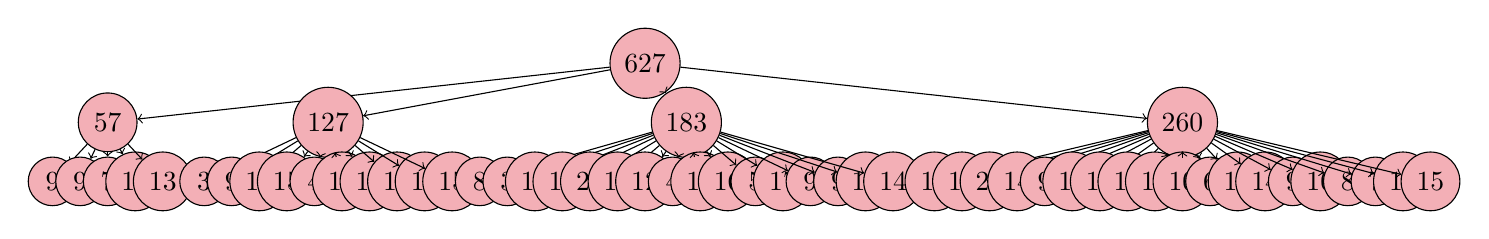
\begin{tikzpicture}[nodes={draw, circle,fill=pink!50}, ->,sibling distance=.7cm,minimum size=.1cm,scale=.5]
 
    \node{627}
        child { node {57}
            child {node {9}} 
            child {node {9}} 
            child {node {7}} 
            child {node {17}}
            child {node {13}}}
        child [missing]
        child [missing]
        child [missing]
        child [missing]
        child [missing]
        child [missing]
        child [missing]
        child { node {127} 
            child {node {3}} 
            child {node {9}} 
            child {node {19}} 
            child {node {15}}
            child {node {4}}
            child {node {17}} 
            child {node {15}} 
            child {node {19}} 
            child {node {11}}
            child {node {15}}}
        child [missing]
        child [missing]
        child [missing]
        child [missing]
        child [missing]
        child [missing]
        child [missing]
        child [missing]
        child [missing]
        child [missing]
        child [missing]
        child [missing]
        child { node {183} 
            child {node {8}} 
            child {node {3}} 
            child {node {12}} 
            child {node {16}}
            child {node {20}}
            child {node {18}} 
            child {node {12}} 
            child {node {4}} 
            child {node {12}}
            child {node {16}}
            child {node {5}}
            child {node {17}} 
            child {node {9}} 
            child {node {9}} 
            child {node {10}}
            child {node {14}}}
        child [missing]
        child [missing]
        child [missing]
        child [missing]
        child [missing]
        child [missing]
        child [missing]
        child [missing]
        child [missing]
        child [missing]
        child [missing]
        child [missing]
        child [missing]
        child [missing]
        child [missing]
        child [missing]
        child [missing]
        child { node {260} 
            child {node {17}} 
            child {node {17}} 
            child {node {20}} 
            child {node {14}}
            child {node {9}}
            child {node {13}} 
            child {node {18}} 
            child {node {10}} 
            child {node {18}}
            child {node {10}}
            child {node {6}} 
            child {node {15}} 
            child {node {14}} 
            child {node {9}}
            child {node {10}}
            child {node {8}} 
            child {node {7}} 
            child {node {13}} 
            child {node {15}}}
            ;
\end{tikzpicture}
    \caption{Example of Hierarchical Clustering for 627 projects}
    \label{fig:example tree}
\end{figure*}
}

\section{Performance Measures}
\label{sec:Measures}

In this section, we introduce the following 5 evaluation measures used in this study to evaluate the performance of machine learning models. Suppose we have a dataset with M changes and N defects. After inspecting 20\% LOC, we inspected m changes and found n defects. Besides, when we find the first defective change, we have inspected k changes. Then the 5 evaluation measures are defined and computed as follows:

(1) \textbf{Recall:} Proportion of inspected defective changes among all the actual defective changes. This is the evaluation measure used by many previous studies~\cite{kamei2012large,yang2016effort,yang2017tlel,xia2016collective,yang2015deep} . They focused on achieving high Recall so that more defective changes could be detected. Recall is computed as: $n/N$.

(2) \textbf{Precision:} Proportion of inspected defective changes among all the inspected changes. A low Precision indicates that developers would encounter more false alarms, which may have negative impact on developers' confidence on the prediction model. Precision is computed as: $n/m$.

(3) \textbf{pf:} Proportion of all suggested defective changes which are not actual defective changes among all the suggested defective changes. A high pf suggests developers will encounter more false alarms which may have negative impact on developers' confidence on the prediction model.

(4) \textbf{popt20:} Proportion number of suggested defective changes among all suggested defective changes, when when 20\% LOC modified by all changes are inspected. A high popt20 indicates that, under the same number of LOC to inspect, developers developers will find more bugs, which means developers will be able to fix more defects with same amount of effort invested.

(5) \textbf{ifa\_auc:} Number of Initial False Alarms encountered before we find the first defect. Inspired by previous studies on fault localization~\cite{parnin2011automated,kochhar2016practitioners,xia2016automated}, we assume that if the top-k changes recommended by the model are all false alarms, developers would be frustrated and are not likely to continue inspecting the other changes. For example, Parnin and Orso ~\cite{parnin2011automated} found that developers would stop inspecting suspicious statements, and turn back to traditional debugging, if they could not get promising results within the first few statements they inspect. ifs is computed as: k. In this study we use a modified version of ifa called ifa\_auc, which calculates ifa based on efforts spent on inspecting the code. We use gradually increment the efforts spent by increasing the total LOC inspected and calculate ifa on each iteration to get the area under the curve (auc), here the x-axis is the percentage of effort spent on inspection and y-axis is ifa.


\section{Results}
\label{sec:results}



\subsection*{RQ1: Can we confirm bellwether on large datasets?}
\label{sec:rq1}

In the literature, we saw most of the previous studies has shown bellwether effect with very small datasets. In order to use bellwether to prove presence of generality in SE domain datasets, we first have to showcase the bellwether method suggested by Krishna et al. in their experiment works for large datasets. We use our defect prediction dataset with 697 projects for this purpose. 

We divide the dataset in train\_1 and test\_1 set and then performed a $ N*(N-1) $ comparison on all the projects in train\_1 set to find a bellwether, and then dividing each project in test\_1 set into train\_2 and test\_2 using a train\_test split. We use the train\_2 to train a LR model and test on test\_2 which is represented as \textit{self\_0} in the figures. Similarly we use the bellwether project from train\_1 to train a LR model and test it on test\_2 which is represented as \textit{bellwether0}. We use statistical tests mentioned in section~\ref{stats} to compare the performance of \textit{self\_0} vs \textit{bellwether0} for all the performance measures mentioned in section~\ref{sec:Measures}, which is shown in figure~\ref{fig:Statistical}. 

It is evident that using the \textit{bellwether method} proposed by Krishna et al. we were able to find bellwether effect in large dataset with 697 projects. This answers this RQ and creates the baseline results for our study. In this RQ1 although we are able to find \textit{bellwether effect}, this method is very expensive, requiring a $ N*(N-1) $ comparison, which in our experimental setup took nearly 3 days of computation. Which takes us to the next research question. In summary, we find that 

\begin{result} {Bellwethers are found when studying over 697 software projects. However, conventional methods of Krishna et al~\cite{krishna2017learning} take far too long to discover these bellwethers, e.g., experimentation took 3 days to find a bellwether project from among the 697 projects.}
\end{result}

\subsection*{RQ2: How to tame complexity of bellwether?}
\label{sec:rq2}

To tame complexity of bellwether in this RQ, we propose a new bellwether method called ``BUBBLE'' to find bellwether in large datasets. This bellwether method is composed of 6 stages, (a) a feature extraction process to summarize each project into a single representative vector, (b) a hierarchical clustering algorithm, which uses the feature vectors to cluster similar projects into community of increasing size at different levels of cluster, (c) a bellwether selection phase where a $N*(N-1)$ comparison is performed at each leaf level cluster and using a cdom calculation in all the metrics mentioned in~\ref{tbl:metric} a bellwether is selected, (d) a iterative bellwether promotion stage, where bellwether from child clusters are promoted as potential bellwethers at parent cluster, (e) another bellwether selection phase at non-leaf levels, where comparisons are only made among potential bellwethers from leaf node and finally (f) a bellwether prediction phase, which suggests a bellwether based on project similarity when a new project is to be predicted. The details of each phase is mentioned in sec~\ref{BUBBLE}. 

In the \textit{bellwether method} proposed by Krishna et al. if there are N projects in a community it will make $\approx N^2$ comparisons to discover the bellwether. While ``BUBBLE'' different approach to discover bellwether by dividing the data into smaller cluster and finding bellwether among each, here if we assume we have m cluster at leaf level with N projects in each, we will have 
$\approx m*(N/m)^2$ comparisons to discover the bellwether which is m times less comparison. For example if we see the example figure~\ref{fig:example tree} for hierarchically cluster a community of 627 projects, if we use the default \textit{bellwether method} it will require \textbf{393129} comparisons. While if we use the ``BUBBLE'' algorithm to find the bellwether it will require only \textbf{9080} comparisons. Using this process we are able to find bellwether in ~\textbf{1.5 hours}, which is order of magnitude faster then the bellwether method proposed by Krishna et al. In summary, we find that

\begin{result}
{``BUBBLE'' can find ``Bellwether Project'' order of magnitude faster, only requiring 1.5 hours in comparison to 3 days. Also ``BUBBLE'' requires far less comparison 9080 instead of 393129 required for ``Bellwether method'' proposed by krishna et al. }
\end{result}

\begin{equation}
\label{eq:bellwether}
    Bellwether\_complexity  \approx O(N^2)
\end{equation}

\begin{equation}
\label{eq:BUBBLE}
    BUBBLE\_complexity \approx O(m*(N/m)^2)
\end{equation}


\begin{figure}
    \centering
    \includegraphics[width=\linewidth]{figs/time.png}
    \caption{Runtime for default bellwether and BUBBLE.}
    \label{fig:time}
\end{figure}





%%%%%%%%%%%%%%%%%%%%%%%%%%%%%%%%%%%%%%%%%%%%%%%%%%%%%%%%%%%
%%%%%%%%%%%%%%%%%%%%%%%Latex Table%%%%%%%%%%%%%%%%%%%%%%%%%
\begin{figure}[!t]
{\small
{\small \begin{tabular}{p{.1cm}lp{1.5cm}rrc}
\arrayrulecolor{darkgray}
\rowcolor[gray]{.9}  & rank & treatment & mean & sd & \\
 \multirow{5}{*}{\rotatebox[origin=c]{90}{Recall}} &   1 &      random2 &    40 &  49 & \quart{16}{40}{49}{25} \\
  &   1 &      BUBBLE\_level2 &    38 &  32 & \quart{22}{38}{32}{16} \\
  &   1 &      bellwether0 &    39 &  31 & \quart{23}{39}{31}{15} \\
  &   2 &      BUBBLE\_level1 &    48 &  33 & \quart{31}{48}{33}{16} \\
  &   3 &      BUBBLE\_level0 &    56 &  31 & \quart{42}{56}{31}{16} \\
  &   3 &      self\_0 &    55 &  27 & \quart{41}{55}{27}{12} \\
  &   4 &      global2 &    78 &  40 & \quart{57}{78}{40}{20} \\ \hline
\multirow{5}{*}{\rotatebox[origin=c]{90}{Pf}} &    1 &      random2 &    39 &  49 & \quart{15}{39}{49}{25} \\
  &  1 &      random2 &    39 &  49 & \quart{15}{39}{49}{25} \\
  &  1 &      BUBBLE\_level2 &    28 &  28 & \quart{14}{28}{28}{13} \\
  &  1 &      bellwether0 &    28 &  25 & \quart{15}{28}{25}{11} \\
  &  1 &      self\_0 &    30 &  20 & \quart{20}{30}{20}{10} \\
  &  1 &      BUBBLE\_level1 &    35 &  28 & \quart{21}{35}{28}{14} \\
  &  2 &      BUBBLE\_level0 &    47 &  31 & \quart{31}{47}{31}{15} \\
  &  3 &      global2 &    79 &  39 & \quart{59}{79}{39}{19} \\\hline
\multirow{5}{*}{\rotatebox[origin=c]{90}{Precision}} &   1 &      random2 &    21 &  30 & \quart{6}{21}{30}{15} \\
    &  2 &      global2 &    35 &  28 & \quart{21}{35}{28}{14} \\
    &   2 &      bellwether0 &    40 &  33 & \quart{23}{40}{33}{16} \\
    &   2 &      BUBBLE\_level2 &    39 &  34 & \quart{22}{39}{34}{17} \\
    &   2 &      BUBBLE\_level1 &    42 &  31 & \quart{26}{42}{31}{15} \\
    &   2 &      BUBBLE\_level0 &    44 &  30 & \quart{28}{44}{30}{15} \\
    &   2 &      self\_0 &    50 &  30 & \quart{35}{50}{30}{15} \\\hline
\multirow{5}{*}{\rotatebox[origin=c]{90}{Popt20}} &   1 &      random2 &    13 &  16 & \quart{5}{13}{16}{8} \\
  & 2 &      BUBBLE\_level2 &    26 &  22 & \quart{15}{26}{22}{11} \\
  &  2 &      global2 &    26 &  13 & \quart{19}{26}{13}{6} \\
  &  2 &      bellwether0 &    28 &  21 & \quart{17}{28}{21}{9} \\
  &  2 &      BUBBLE\_level0 &    28 &  15 & \quart{22}{28}{15}{8} \\
  &  2 &      BUBBLE\_level1 &    28 &  19 & \quart{19}{28}{19}{9} \\
  &  3 &      self\_0 &    35 &  19 & \quart{26}{35}{19}{10} \\\hline
\multirow{5}{*}{\rotatebox[origin=c]{90}{ifa\_auc}} &   1 &      random2 &    7 &  11 & \quart{1.12}{6.77}{11.29}{5.65} \\
  &  2 &      global2 &    19 &  16 & \quart{11.35}{19.38}{16.06}{8.03} \\
  &  3 &      BUBBLE\_level2 &    22 &  14 & \quart{14.48}{21.59}{14.21}{7.10} \\
  &  3 &      bellwether0 &    23 &  14 & \quart{15.48}{22.56}{14.15}{7.07} \\
  &  3 &      self\_0 &    23 &  12 & \quart{17.09}{22.93}{11.68}{5.84} \\
  &  3 &      BUBBLE\_level1 &    23 &  14 & \quart{16.10}{22.98}{13.74}{6.87} \\
  &  3 &      BUBBLE\_level0 &    25 &  13 & \quart{17.87}{24.51}{13.27}{6.63} \\
\end{tabular}}
}
\caption{Statistical Results comparison
}\label{fig:Statistical}
\end{figure}
%%%%%%%%%%%%%%%%%%%%%%%End Latex Table%%%%%%%%%%%%%%%%%%%%%
%%%%%%%%%%%%%%%%%%%%%%%%%%%%%%%%%%%%%%%%%%%%%%%%%%%%%%%%%%%





\subsection*{RQ3: Is faster bellwether effective?}
\label{sec:rq3}

In RQ2, we can see using ``BUBBLE'' we are able to find bellwether for a large dataset in order of magnitude faster. This raises the question is  \textit{bellwether method} ``BUBBLE'' as effective as \textit{bellwether method} proposed by krishna et al. and can it be compared against local(self test) and global models? 

To answer this question in this study we have used the defect prediction dataset with 697 projects and divided the projects randomly into train\_1 and test\_1 as a 90-10 split, the projects in train\_1 was used to find the bellwether in each cluster in the CF Tree as mentioned in sec~\ref{BUBBLE}, and then each project in test\_1 was divide into train\_2 and test\_2 split. We trained a LR model using train\_2 for each project and tested on test\_2 (represented as self\_0), this is represented as self test in this study. We also used the predict stage of the ``BUBBLE'' to identify a bellwether in each level of hierarchical model, for each project in test\_1 and tested the performance on test\_2 (represented as bellwether\_level0, bellwether\_level1, bellwether\_level respectively). Similarly we used the projects in train\_1 to find the bellwether using default bellwether method as mentioned in sec~\ref{Bellwether}, and use that project to build a LR model and test the performance of each project's test\_2 (represented as bellwether0). And we combined all the data from train\_1, and used that to build a global model and tested on test\_2 (represented as global2). We compare the performance of each model described above using statistical tests as mentioned in section~\ref{stats} and if 2 models are ranked different that represents their performance is significantly different. 

We can see from the figure~\ref{fig:Statistical} that bellwether\_level0 model (i.e. the bellwether discovered by ``BUBBLE'' at level 0) performs similar or  better than bellwether0 in most of performance metrics. Similarly for self\_0 in terms of precision, recall and ifa\_auc bellwether\_level0 scores same rank using statistical significance and effect size test. Although for bellwether0 and self\_0 the performance rank for pf and Popt20 is little better than bellwether\_level0, the difference is very small. We can see similar results for the global2 results, where bellwether\_level0 performs significantly better. Seeing these results we can conclude the ``BUBBLE'' is an effective and fast algorithm to find a exemplary ``Bellwether Projects'', whose predictive performance is comparable with  \textit{bellwether method} proposed by krishna et al. , local(self test) and global models. In summary, we find that

\begin{result}
{``BUBBLE'' is a fast and effective algorithm, which can find exemplary ``Bellwether Projects'' with comparable predictive performance.}
\end{result}




\subsection*{RQ4: Does learning from too many projects has detrimental effect?}
\label{sec:rq4}
In RQ4, we try to answer the question if learning from too many projects detrimental effect, this question has two parts one on predictive power, other on making general conclusion and conclusion instability. Figure~\ref{fig:Statistical} show the results of statistical significance and effect size tests to rank them in order for all the different methods(treatments) used in this experiment. In this figure for a performance measure two methods showing same rank means there performance is not statistically significantly different, while a different ranks means they are different, while a smaller rank is better if the performance goal is negative (i.e. Pf), and higher rank is better in case of positive goal (i.e. Recall).

To answer the first part of the question, if learning from too many projects have detrimental effect on predictive power of models, we compare the results of default ``bellwether method'' (a.k.a bellwether0) proposed by krishna et al. and ``BUBBLE''(a.k.a BUBBLE\_level0) method. The results of scott-knott test shows that for positive goals such as Recall the BUBBLE\_level0 is significantly doing better than Bellwether0 and it is doing as good as or better for precision ans recall. While for negative goals such as ifa\_auc BUBBLE\_level0 is doing as good as bellwether0. Although in case of Pf they score different ranks with BUBBLE showing higher Pf then bellwether0, it is not by much. Similarly while comparing BUBBLE\_level0 with global (which is learning from all the projects) shows although it achieves higher Recall, but it has very high Pf, low precision. Which answers the first part of the question that learning from too many projects do have detrimental effect on predictive power of models. 

\begin{table}[!t]
\centering
\caption{Importance of coefs on \textit{log p} from logistic regression model of ``Bellwether'' shown in fig~\ref{fig:FSS_compare}. Here Odds ratio shows one increment in in respective variable increase in the log-odds of being defective.}
\begin{tabular}{|l|l|l|l|} \hline
Rank & Attr               & coef  & Odds ratio \\ \hline
1    & avg\_NPRM          & 2.23  & 9.26      \\ \hline
2    & avg\_NPBM          & -1.31 & 0.27      \\ \hline
3    & max\_NPBM          & -1.12 & 0.33      \\ \hline
4    & max\_RFC           & 0.74  & 2.09      \\ \hline 
5    & total\_NPBM        & -0.70 & 0.50      \\ \hline
6    & max\_CBO           & -0.64 & 0.53      \\ \hline
7    & total\_ModifiedLOC & 0.10  & 1.10      \\ \hline
8    & avg\_WMC           & 0.07  & 1.07     \\ \hline
\end{tabular}
\label{tbl:coefs}
\end{table}

Now to answer the second part of the question, that is if learning from too many projects creates conclusion instability, we will look at the figure~\ref{fig:FSS_compare}. Figure~\ref{fig:FSS_compare} show the distribution of attributes selected while building a ML model for defect prediction using local models(a.k.a self\_0), the \textcolor{red}{{\bf red bars}} shows the attributes selected by the ``Bellwether Project''. Conclusion instability causes vastly different and often contradicting conclusions to be derived from a data source. This sort of instability is very prevalent in several domains of software engineering. We can see from figure~\ref{fig:FSS_compare}, when learning from local data, each model selected different sets of attributes and resulted in selecting almost all different attributes. That means there is no general conclusion can be drawn for defect prediction models by saying which attributes are important, this results in conclusion instability and that effects the trusts on those models, the insights that can be drawn from them. Which farther affects training and tool development as mentioned in sec~\ref{sec:Motivation}. From these results we can see learning from too many data can cause conclusion instability and thus affecting generality in SE domain. In Summary, we can say 

\begin{result}
{Learning from too many projects have detrimental effect on predictive power, which can be seen on performance difference found between bellwether0 and BUBBLE\_level0, it also introduces conclusion instability. By selecting ``Bellwether Project'' using BUBBLE can have better predictive performance as well as it can create generalized model which are explainable and actionable thus minimizing conclusion instability.}
\end{result}

\begin{figure*}[h]
    \centering
    \includegraphics[width=\linewidth]{figs/FSS_compare.png}
    \caption{Distribution of attributes selected using self\_0 model and ``Bellwether'' model.}
    \label{fig:FSS_compare}
\end{figure*}

\subsection*{RQ5: What did we learn?}
\label{sec:rq5}

In this RQ we show what did we learn by selecting a ``Bellwether Project'' to create defect prediction models. Using ``Bellwether Project''  minimizes the issue of conclusion instability and thus building trust in the model and deduce better insights about what can be a better indicator of bugs. Table~\ref{tbl:coefs} show the attributes selected by the ``Bellwether Project'' and the coefs and Odd ratios for the LR model build using that. The insights that we can draw from these results are an increase of 1 in avg\_NPRM can increase the ratio of probability of having a defect and not having a defect by almost 9 times, while an unit increase in total\_NPBM, avg\_NPBM, max\_NPBM, max\_CBO will reduce the ration of probabilities by 0.5, 0.27, 0.33 and 0.53 times respectively. an unit increase in total\_ModifiedLOC and avg\_WMC will have almost no effect in Odd ratio. From this we can conclude NPRM, NPBM, RFC and CBO are important factor while predicting for defects all of which are interface related metrics in these datasets. The learning from these information can be if there is increase in number of private methods in a certain class, developers need to be extra careful as that is a good indicator of introducing bugs in code. In Summary, we can say 

\begin{result}
{Learning from ``Bellwether Project'' is very concise, can be used to extract meaningful and actionable insights. The insight from this study is interface related metrics collected from these 697 projects are good indicator of bugs in the codebase. }
\end{result}


\section{Threats to Validity}
\label{sec:validity}

As with any large scale empirical study, biases can affect the final
results. Therefore, any conclusions made from this work
must be considered with the following issues in mind:

(a) \textit{Evaluation Bias}: 
In  RQ1, RQ2 and RQ3 we have shown the performance of local model, hierarchical bellwether models, default bellwether model and compared them using statistical tests on their performance to make conclusion about presence of generality in SE datasets. While those results are true, that conclusion is scoped by the evaluation metrics we used to write this paper. It is possible that, using other measurements, there may well be a difference in these different kinds of projects. This is a matter that needs to be explored in future research.  

    
(b) \textit{Construct Validity}: At various places in this report, we made engineering decisions about (e.g.) choice of machine learning models, hierarchical clustering algorithm, selecting feature vectors for each project. While those decisions were made using advice from the literature, we acknowledge that other constructs might lead to different conclusions. 

(c) \textit{External Validity}: For this study we have relied on data collected by zhang et al.~\cite{zhang15} for their studies. The metrics collected for each project was done using an commercialized tool called ``Understand''. There is a possibility that calculation of metrics or labeling of defective vs non-defective using other tools or methods may result in different outcome. That said, the ``Understand'' is a commercialized tool which has detailed documentation about the metrics calculations and zhang et al. has shared their scripts and process to convert the metrics to usable format and has described the approach to label defects.  

We have relied on issues marked as a `bug' or `enhancement' to count bugs or enhancements, and bug or enhancement resolution times. In Github, a bug or enhancement might not be marked in an issue but in commits. There is also a possibility that the team of that project might be using different tag identifiers for bugs and enhancements. To reduce the impact of this problem, we  did take precautionary step to (e.g.,) include various tag identifiers from Cabot et al.~\cite{cabot2015exploring}. We also took precaution to remove any pull merge requests from the commits to remove any extra contributions added to the hero programmer. 

(d) \textit{Statistical Validity}: To increase the validity of our results, we applied two statistical tests, bootstrap and the a12. Hence, anytime in this paper we reported that ``X was different from Y'' then that report was based on both an effect size and a statistical significance test.
 
(e) \textit{Sampling Bias}: Our conclusions are based on the 697 projects collected by zhang et al.~\cite{zhang15} for their studies. It is possible that different initial projects would have lead to different conclusions. That said, this sample is very large so we have some confidence that this sample represents an interesting range of projects. As evidence of that, we note that our sampling bias is less pronounced than other ``Bellwether'' studies since we explored.
 



\section{Conclusion}
\label{sec:concl}
In this paper, we have proposed a new transfer learning ``bellwether method'' to find ``Bellwether effect'' called ``BUBBLE'' and uses this to find generality in Software Engineering by minimizing conclusion instability thus increasing trust and deducing meaningful insights from them which in turn helps in training and tool developments. 

Our results show that regardless size of software engineering datasets we can still find ``Bellwether'' in those datasets. In this study bellwethers were found when studying over 697 software projects. However, conventional methods of Krishna et. al. are computationally very expensive and took long time to discover these bellwethers, e.g.,experimentation took 3 days to find a bellwether project from among the 697 projects.

We showed in this paper, the new algorithm ``BUBBLE'' can find ``Bellwether Project'' order of magnitude faster. We show ``Bellwether method'' proposed by krishna et al. has a computational complexity of $\approx O(N*2)$ while ``BUBBLE'' has a computational complexity of $\approx O((N*2/m))$ where m is the number of cluster at the leaf level of the CF tree and N is the number of projects. ``BUBBLE'' only requiring 1.5 hours to run in comparison to 3 days and requires far less comparison 9080 instead of 393129 required for ``Bellwether method'' proposed by krishna et al.

The study also showed the ``BUBBLE'' is a fast and effective algorithm, which can find exemplary ``Bellwether Projects'' with comparable predictive performance. The figure~\ref{fig:Statistical} shows ``Bellwether Projects'' discovered by ``BUBBLE'' have similar or better predictive performance while comparing with bellwether0, Self\_0 or global2. 

We also try to answer the question if learning from too many projects have detrimental effect, the study showed it can have detrimental effect on predictive performance of models also it introduces conclusion instability. We can see local models(a.k.a self tests) although having almost similar predictive performance does not allow us to draw general conclusions and insights for software defect prediction models. Thus it is very unlikely users will be able to trust these models and uses them for training, tool development and other related activities. Contrast to that, using a ``Bellwether Project'' we are able to make general conclusion about software defect prediction models. 
 
Hence, from a  engineering perspective there are two main reasons to use ``BUBBLE'': (a) This is a very fast algorithm to find ``Bellwether project'';  (b) They have comparable predictive performance than its counter parts; and (c) They slow down the pace of conclusion changes and allow users to draw generalized conclusions and meaningful actionable insights .

Finally, we remark that much of the prior work on homogeneous transfer learning have complicated the homogeneous transfer learning process and are computationally expensive. We strongly recommend that when building increasingly complex and expensive  methods, researchers should pause and compare their supposedly more sophisticated method against simpler alternatives. Going forward from this paper, we would recommend that the transfer learning community uses ``BUBBLE'' as a baseline method against which they can test more complex methods.

% \section{Future Work}
% \label{sec:furute}



\section{Acknowledgements}
\label{sec:ack}


\bibliographystyle{IEEEtran}
\bibliography{main} 
\clearpage

% %%%%%%%%%%%%%%%%%%%%%%%%%%%%%%%%%%%%%%%%%%%%%%%%%%%%%%%%%%%%%%%%%%%%%%%%%%%%%%%%
%                               RESPONSE TO REVIEWERS
%%%%%%%%%%%%%%%%%%%%%%%%%%%%%%%%%%%%%%%%%%%%%%%%%%%%%%%%%%%%%%%%%%%%%%%%%%%%%%%%

\pagebreak
\newpage
\renewcommand*{\thesection}{\Alph{section}}
\nobalance
\section*{RESPONSE TO REVIEWERS}
\section*{Comments from the editor}

\review{I would like to thank the authors for submitting their work to TSE. While all the reviewers agree that the problem addressed is important and the paper has potential, the reviewers also identified several concerns that need to be carefully addressed. The reviewers also agreed that the amount of work needed to address those concerns is beyond a major revision. Thus, after carefully checking the reviewers and in accordance with reviewer’s recommendations, I also recommend “Revise and resubmit as New”.}

\response{ Thank you very much for your encouraging comments. We have made appropriate changes to the manuscript taking into careful consideration the recommendations of the reviewers. We hope that this new draft adequately satisfies all the issues raised by the reviewers. To assist the reviewers in tracking all the new changes, where appropriate, we have prefixed the text with \respto{X-XX} to correspond to the reviewers' questions.~\\
Below is the brief summary of our changes:
\be
\item The problem statement has been  clarified and properly positioned (R1, R3). XXX
\item The novelty of the approach has  been clarified (R3). XXX (see \bareresp{2-1})
\item Using comments from  (R1, R2, R3), we have made numerous small editorial improvements.
\item The study now includes all the details to ensure replicability (R1, R2).
\item The results of the study need to be revisited since the reviewers are not convinced that the results support the claims in the paper (R1, R2, R3).
\item The background on transfer learning has been augmented with more  citations (R2).
\ee}


\section*{Reviewer 1}

\response{Thank you very much for your detailed review. We have made some additional corrections, clarifications, and revisions, as directed by your comments. To assist in your review, we refer to specific locations of each of the changes using \respto{1-XX}.}

\review{(1.1) Background. The paper builds upon a number of previous studies. However, several key questions have no answer: *What is* the bellwether? *Why is* this relevant? How does it work when applied to different contexts? Why is this useful in practice?}

\response{You are quite correct, we did not define bellwether till very late in the prior draft. In this draft, we define bellwether on page 1.
}

\review{The paper mentions that: "The core intuition of this new approach is that if many projects are similar, then we do not need to run comparisons between all pairs of projects": very good, but where this intuition come from?}


\response{Thank you for that comment.  You a re quite correct-- we did not document the source of our intutuion. We have added the following note to \respto{1-XX}}

\begin{quote}
\response{``The core intuition of this new approach is two-fold. Firstly,
many projects are similar in structure. We say this since  Devanbu
et al.`\cite{hindle2012naturalness}   report that if Markov chains are created for tokens in a program,
then a remarkably small number of chains capture most of the program. ~\\
``Secondly, given these similarities,   we can exploit symmetries between different projects in order to learn predictors from one and apply those to another. To say that anothe way, given large scale similarities between projects,  then we do not need to run comparisons between all pairs of projects since analyszing just a few pairs should work as well as anything else.''}
\end{quote}
 

\review{(1.2)The relevance of the paper. This is, unfortunately, unclear. According to the abstract and introduction, the main issue treated in the paper is related to scalability. Please, provide a clear case study on the performance of bellwether methods. The claims on the scalability of the approaches are just claims, no details are reported. Abstract and introduction just report that "when applied to the 697 projects studied here, they took 60 days of CPU to find and certify the bellwether". As said, the bellwether approach has been applied to several problems (e.g., defect prediction/effort estimation/bad smell detection): are these problems the same? When is it needed to apply scalable solutions for bellwether approaches? Why? Please, explain.}

\response{ need a new RQ0: how slow is standard bellwether. theoretically an empriically its slow (chart on p2. move to RQ0). May need to include results using increasing community size.}

\review{(1.3) Writing style. The introduction is, simply, to be completely rewritten. I would like to see a paper that is understandable even from non-experts. As such, please define the context of the paper, the concepts of (1) software quality - line 1, (2) general models - line 2, (3) many projects - line 2, (4) "scalable approach to learning effective models adapted to the task at hand" - line 2/3, (5) "or does the truth lie somewhere in-between" - line 3. These are just of the examples of why the introduction is unclear and does not provide any detail on the reasons behind the paper. The same is true for the remaining of the paper, which gives for granted many of the concepts without explaining them properly.}


\response{ frist 3 oaras deled tup to :"funding general lessons"}

\review{(1.4) Please, avoid claims such as "have tremendous practical significance" without providing any practical significant example/citation. (This is just an example)}

\response{ you are right. sueprlatives deleted (including that one)"}


\review{(1.5a) The clarity and replicability of the paper are unclear. Here some examples 1) "The logistic regression learner (since it is relatively fast)". What does "fast" mean? How was "fast" computed? }

\response{ you are right. sueprlatives deleted (including that one)"}


\review{(1.5b)
2) "The SMOTE class imbalance correction algorithm [49], which we run on the training data2". Why is SMOTE needed? Why is the problem unbalanced? Please, explain.
}

\review{(1.5c)
3) "and Hall’s CFS feature selector". Which features have been removed and why?
}

\review{(1.5d)
4) "As to CFS, we found that without it, our recalls were very low and we could not identify which metrics mattered the most". Where can the reader understand this statement? Where is the replication data? }

\response{how should I answer Where can the reader understand this statement? May need to remove this section as i don't have the results}


\review{(1.5e)
5) "extensive studies have found that CFS more useful than many other feature subset selection methods such as PCA or InfoGain or RELIEF". The paper cites just one paper, how should these studies be "extensive"? }

\response{Thank you for that comment.  You are quite correct-- we did not document the all the necessary citations for supporting our claim before. We have added the following note to \respto{1-5e}}

\review{(1.5f)
5) "Maximize recall and precision and popt(20)": Why should these metrics be maximized? What is the practical value, e.g., is high recall always needed in practice, or should we prefer precision in the problems treated by the bellwether? What about popt(20)?}

\response{added footnote also there are details in sec 4.5}


\review{(1.5g) "While minimizing false alarms and ifa auc": Again, please explain the practical relevance of the performance metrics employed. }

\response{added footnote also there are details in sec 4.5}


\review{(1.5h) 
More in general, how can one replicate the performed study? Is there a replication package? If so, where?}

\response{Thank you for that comment. You are quite correct-- we did not include in depth steps to replicate the study before. We have added a replication package in contribution section \respto{1-5h} as well as more in depth details about the algorithm has been added in \respto{XXXX}}

\review{(1.6a) The analysis of the results should be substantially improved. Let consider the case of Section 5 - RQ1. The results are reported in less than half column and refer to a figure (Figure 6) which does not explain anything. The summary reports that "Theoretically and empirically, the hierarchical reasoning on GENERAL performs much faster than standard bellwether methods": I cannot understand where these "theoretically and empirically" come from, since there is no proof of them. }

\response{you are wright, need an RQ0}

\review{(1.6b)
The same is true for the other research questions. And, in general, there is qualitative analysis: Why are the results the ones reported in the paper? }

\response{you are right,Thank you for that comments. We have added much  quantaitive analusis as
well as statistical tests to this paper. Please see \fig{XXX7}.}

\review{(1.6c) What makes the reported method scalable?}

RQ0: how slow old better

RQ1: how fast new bellweather.

RQ2: scalabulity (the old RQ1)

RQ3: (as before)

RQ4: (as belfire)



\section*{Reviewer 2squeue}

Many of your comeents take issue with two terms used in this paper "lessons learned" and "trasfer learning".
We agree with you that our use of "lessons learned" was inappropriate and we have removed all those usages.

As to oir use of "transfer learning", 
inspired by your commetns we have ckarified what we mean by that term much earlier in the paper (see \cite{XXX}). Base don that clarification, we can show that our use of ``transfer learning'' is consistent with its usage by Pan'09 (a paper current 8,220 citations at the time of this writing). Also, our usage is consistent with dozens of recent SE research papers on transfer learning~\cite{XXXmanycite}. Thank you for enocuraging us to clarify that terminology.

A survey on transfer learning
SJ Pan, Q Yang - IEEE Transactions on knowledge and data …, 2009 - ieeexplore.ieee.org
  Cited by 8220 Related articles All 20 versions Web of Science: 3428
  


% \review{(2.1) [Sec. 1 and throughout] The paper repeatedly refers to a method for “transferring lessons learned from one project to another.” But the method does NOT transfer lessons learned. Lessons learned are identified throughout and formally documented in the project closing process.}

% \response{ u r right. lessons learned are what yu said. what we do pass pom
% defect predictors from one project to another (and this passage process of data mining results is very different to the lessons learned process you describe).   }

% \review{These lessons learned are reviewed when new projects are being initiated/planned. The introduction talks about guiding project management but project management has a process for handling lessons learned that doesn’t require machine learning. How does the method help that process? Why would you need a “bellwether” to apply lessons learned to a new project?! The method does not transfer lessons learned but what it DOES appear to do is associate defect rate profiles for two projects (a so-called “bellwether” and a new project).}


% \response{ ur rught we renamed as you said. }

\review{(2.2) [Sec. 1] “…the bellwether is equivalent to the other models…” This claim is confusing. 1) Is “the bellwether” a model or a project? 2) How is equivalence defined? Or do you simply mean “similar”?}

\response{ acts as data poasss on. cjanged to similiar.}

\review{(2.3) [Sec. 1] “when new projects appear, their quality can be evaluated even before there is an extensive experience base within that particular project (again, just by studying the bellwether).” You take a set of projects…select one project (the “bellwether”)…then use that project to build a model that can—for instance—estimate defect rate. So, for the defect estimation case, the model learned from the bellwether won’t tell you where the defects may be (i.e., fault localization), it will just estimate how buggy a new project is. Is all of this right?}

\response{ XX.}



\review{(2.4) If the point is to use the bellwether to infer things about a “new” project, then how new can the new project be? When (in the new project’s history) can you be sure the model from the bellwether is valid to use?}

\response{Explain the train, test splits and the how you do the exp. then say this is what our model proves, it predicts for projects which it has not seen before XX.}

\review{(2.5) Do you have to find a bellwether for each purpose? In other words, if you find a bellwether among 697 projects for defect rate prediction, then is that same bellwether automatically used to build a model for another discrete task (different than defect rate prediction)? Or will you have to apply this algorithm for each and every discrete task?}

\response{ clairft}

\review{(2.6) Figure 1 needs to be omitted}

\response{ ciuretainly too confusing for intro. can move to a later section and ducssed in more retchnical detail}

\review{(2.7) The computational complexity $(O(N^2)$ versus $O(m*(N/m^2))$ is both compact appropriate.}

\response{ XXXX}

\review{(2.8) The paper does not evaluate the model’s performance using a pool of 12,000 projects; the evaluation does not even use 1,000 projects.}

\response{ will fix}


\review{(2.9) [Sec. 1] The box under RQ4 is very confusing. We find the bellwether to simply study one project, but this note says we still need to analyze hundreds of projects to understand something like the importance of features. Is this right?}

\response{ will fix}

% \review{(2.10a) [Sec. 1] The contributions of this paper.
% 1) The first contribution claims “bellwethers for transfer learner.” Indeed, the paper repeatedly refers to transfer learning. But I do not see where the transfer learning is actually being done when I inspect the procedure at the beginning of Sec. 3:}


% \review{(2.10b)
% [A] Step 1 characterizes each project using the same feature space and the paper does not support the fact that data are distributed differently. Moreover, the learning task remains the same. These facts do not support a transfer learning setting prima facia.}

% \response{(2.10c) with respect, our usage is consistent with how the term is used in the SE literature, see LOTS of ferences~\cite{xxx}.}

% \response{(2.10d) 
% [B] Steps 2 and 3 involve grouping the projects based on similarity. There is no transfer learning here.}

% \response{(2.10e) 
% [C] There is no transfer learning done in Steps 4-6.}


% \response{(2.10f) 
% [D] Aside from inspecting each step in the main procedure, another way to determine whether GENERAL involves transfer learning is the following: This approach does not involve reweighting instances nor does it appear to involve transferring feature representations and/or parameters…and if it does then the paper does not even identify this fact much less argue for it being the case.
% If something in this rationale [A-D] is not correct, then please clear up the explanation on transfer learning in the paper in terms/language the machine learning community has established to avoid ambiguity.}


\review{2) I do not understand what the second contribution really is.}

yes, we have deletet is

\review{(2.11) [Sec. 2.1] I recommend removing this subsection from Background and condensing it in the motivation in Sec. 1.}

good idea. paper now starts with 2.1

\review{(2.12) [Sec 2.2] Figure 2 needs to be omitted. These “hypothetical” plots are not substantial. (The authors even say as much when discussing the results in Sec. 5.)}

replaced with two dots poiints: descibning this in wors

\review{(2.13) [Sec. 2.2] At least two-thirds of this sub-section is anecdotal. Does the gist of this subsection depend critically on the hypotheticals?}

get rid of 2.2.. delete fig 2

\review{(2.14) [Sec. 2.3] “Accordingly, here, we explore nearly 700 projects.” But just because 697 (this study) is larger than 24 (previous studies) does not mean external validity concerns are adequately addressed when one considers how complex the task is. Please comment.}

\response{with respect, in terms of SE reserch, it it smuch larger thatnanythtngoins eeen before. but your concenr is valud. we have added
a weaselt sentence at the end saying that we can benever assume generality of all porkect. }

\review{(1.15) [Sec. 2.3] “If they ask ‘are we sure XYZ causes problems?’, can we say that we have mined enough projects to ensure that XYZ is problematic?” We can say XYZ is probably problematic, but that doesn’t answer the deeper question about causality. Do you agree?}

\response{ ur right. we shiuld bneve wsay "cuase'. work removed. is associated, statisitally predicts for.}

% \review{(1.16) [Sec. 2.4] “This art of moving data and/or lessons learned from one project to another is Transfer Learning.” I do not agree with this definition. Please cite this definition or use the definition of transfer learning established by the machine learning community.}

\review{(2.17) [Sec. 2.4] “Successful transfer learning can have two variants…” Cite these variants. This is a software engineering paper—not a machine learning paper—that should reference other work for these fundamental details.}


\response{citations added.}

\review{(2.18) [Sec. 3.2] “…for large sample datasets…” What is the size of the design matrix? Does 21 product metrics and five process metrics mean 26 columns? If there are 697 projects and snapshots every six months, then how many rows are there?}

\response{XXX}

\review{(2.19) [Sec. 3.3] “As discussed below, the defect models assessed in these experiments” Incomplete.}

\response{fixed}

\review{(1.20) [Sec. 4.1] “stratified k=5 fold cross-validation an” Incomplete.}


\response{fixed}

\review{(1.21) [Sec. 5] “To put that another way, the answer to ‘is is [sic] possible to learn from too much data’, is ‘depends on what you value’” How does your concept of learning from too much data relate to the concept of overfitting? Same concept? Different concepts? If so, how are they different?}

\response{timm}

\review{(1.22) [Abstract] “When one exemplar project…offers the best advice then it can be used to offer advice for many other projects.” The word advice is confusing here. The so-called bellwether does not offer advice or recommendations. It is simply used as a characterization, right?}

\response{predicttions}


\review{(1.23) [Sec. 2.3] “…among developers, there is little agreement on what many issues relating to software.” Please reword.}

\response{fixed}

\review{(1.24) [Sec. 2.3(c)] “For example…” is a run-on sentence.}

\review{(1.25) [Sec. 3] What are the units for dataset size in Fig. 4?}

\review{(1.26) [Sec. 5] Why do you need a figure (Fig. 6) for two numbers?}


\section*{Reviewer 3}

\review{(1.1)What I find irritating is that the manuscript introduces a new approach GENERAL, which just applies hierarchical clustering. As far as I understand, hierarchical clustering is a well-known, standard, and largely-evaluated clustering algorithm. I don’t really see the need to rebrand it with a new name. What is the difference between GENERAL and hierarchical clustering other than the GENERAL is applied to defect prediction?}

\review{(1.2) Figure 1 “shows a hypothetical cost comparison in AWS between standard bellwether and GENERAL.” If the Figure is hypothetical, why do we need it? Is it based on real data? As far as I understand, the plot is merely speculation and as such is should be included in scientific papers.}

we will remove

\review{(1.3) I am also very concerned about the (unproven) assumption that we can make conclusions that hold across multiple projects. While the dataset includes 700 projects, we have no information about the project, the domain applications, criticality (e.g., safety-critical systems vs. generic open-source Java libraries). I don’t really see how a model trained on dozens of open-source apache libraries can be applied to robotics, medical systems, etc. Note that for the latter domains, testing, requirements engineering, and maintenance are different and have peculiar standards (e.g., MC/CD coverage for automotive systems vs. statement coverage for non-critical systems). See below further comments about the quality of the dataset.}

wirht respect.... but we can

\review{(3.4) Similar to Figure 1, Figure 2 discussed hypothetical results/comparisons. Why do we need to speculate on hypothetical data rather than real data? The last two paragraphs in Section 2.2 make little sense to me. There is no reason to have them, if not for contributing to the overall overselling.}

fig2 remove

\review{(3.5) Up to page 5 (Sections 1-2), the paper broadly discusses the importance of learning models from hundreds of projects to have more generic and more reliable software analytics in a broader sense. However, from Section 3 to Section 6, the manuscript focuses on defect prediction ONLY.}

sure. tahts oour case study

\review{(1.6) How can we use one single sub-domain (i.e., defect prediction) to make bold statements that should be valid for software analytics in general? This overselling concerns me a lot. This manuscript DOES NOT provide any evidence that GENERAL works and is applicable for other contexts other than defect prediction. In other words, SE is not only Defect Prediction.}

not in general. cant prove external validity. jsut for our 673 projects. wichi is orders of mangitude larger than anything seen ebfore.

\review{(1.7) Therefore, the title, the abstract, introduction, motivation, and conclusions should mention defect prediction as to the only sub-domain in which GENERAL has been evaluated. Any overselling to other domains (or software analytics in a broader sense) should be removed (perhaps mentioned as part of future work) because it is not supported by what is in the empirical study/results.}

we agree. titlte shcnage accouding.


\review{(1.8) As mentioned in one of my comments above, the script seeks to model generalizability looking at the number of projects (and size) as solely dimension to look at. But what about the quality attributes, such as the application domain? What are the application domains of the projects? Are there only open-source projects? How about industrial projects, including the financial, automotive, and robotics sectors? How many web and mobile applications are in the sample? Does the dataset cover these domains? If not, how can we claim that 700 projects can bring us to generalizability?}

not in general. cant prove external validity. jsut for our 673 projects. wichi is orders of mangitude larger than anything seen ebfore.

\review{(1.9) Furthermore, the dataset looks quite strange to me. Looking at the defect distributions (left-most boxplot in Figure 4), I do see that 75\% of the projects (the last quartile) have more than 60\% of defective modules (classes/methods?). Some have a defective percentage above 80\%. Do we need machine learning to predict defects in projects where almost all modules are defectives? In these projects, a simple, constant classifier would work the best. The results also show this for ZeroR in Section 5.}

unclear on this. zeroR tells us that it is not enough to do simple things


\review{(3.10) Throughout the manuscript, the complexity of GENERAL is suggested to be $O(m * (N/m)^2)$. But there is proof about the complexity whatsoever. Either the manuscript cites proofs from existing papers (e.g., related work on hierarchical clustering) or provides a complete proof (perhaps in an appendix).}


XXXX

\review{(1.11) All the results are summarized in one single table (Figure 7), which shows the mean and the standard deviation of five evaluation metrics, as well as the rank of the statistical tests. There are two problems in aggregating the data in this way: (1)I am not sure that the arithmetic mean and the standard deviation are the appropriate metrics to use. Are the data normally distributed? Do we have many outliers? Perhaps, median and IQR are more appropriate as they are less affected by outliers.}

use medians an QRQ

{Maybe, the boxplots would be the most appropriate way to show the distributions. (2)The average across 700 projects makes little sense and hides what happens in each project. What happens per project? In how many projects does GENERAL performs better than the standard bellwether learner?}

xplain

\review{(1.12) Section 5 contains the following recommendation “As to ZeroR, we cannot recommend that approach. While ZeroR makes few mistakes (low ifas and low pfs), it scores badly on other measures (very low recalls and popt(20).” This argument does not convince me as ZeroR gets the best results for two metrics (as far as I understand). Please elaborate more on why we cannot use ZeroR. Besides, ZeroR may work relatively well because of projects with a very large number of defects. Perhaps, some in-depth analysis of the correlation between defect distributions and performances of the models would be very useful.}

Xplan

\review{(1.13) Section 5 (RQ3) ends with two recommendations about critical and non-critical systems. However, I could not find any analysis that can support these recommendations. I also queried the paper looking for the keywords “critical systems,” but I could not find anything except the recommendation with these keywords. To address this, there are only two mutually exclusive solutions: either remove the recommendations or add in-depth analysis that can provide empirical evidence to the claims.}


cget rid of critial systems


\end{document}

